
%% Use the first of the following lines during production to
%% easily spot "overfull boxes" in the output. Use the second
%% line for the final version.
%\documentclass[12pt,draft,letterpaper]{report}
\documentclass[12pt,letterpaper]{report}

% for debugging
%\usepackage{showframe}

% Fncychap is used for fancy chapter headings, but it also gives the formatting commands I needed to define the new 
% \appendixchapter command. You should look at its documentation and pick a nice style to use.
\usepackage{fncychap}
\sloppy

% Appendix allows the inclusion of a line for "appendices", which otherwise won't get the right page number. You must
% use the [toc] option.
\usepackage[toc]{appendix}

% Tocloft is used to create the new list of appendices. You must use the [titles] option.
\usepackage[titles]{tocloft}

% Number the subsubsections and include them in the TOC
\setcounter{secnumdepth}{3}
\setcounter{tocdepth}{3}

% Create list of appendices, and don't include appendices in the table of contents
\newlistof{appendixchapter}{apx}{List of Appendices}

\newcommand{\appendixchapter}[1]{%
    \refstepcounter{appendixchapter}%
    \refstepcounter{chapter}%
    \renewcommand{\DOTIS}[1]{\DOCH \DOTI{#1}}
    \chapter*{#1}
    \addcontentsline{apx}{appendixchapter}{Appendix \protect\numberline{\theappendixchapter}#1}\par%
    \vspace {-1.47cm}}
    
\renewcommand{\theappendixchapter}{\Alph{appendixchapter}}

\newcommand{\appendixsection}[1]{%
    \refstepcounter{section}%
    \section*{\protect{\thesection}\hspace{2.6ex}#1}}
    
\newcommand{\appendixsubsection}[1]{%
    \refstepcounter{subsection}%
    \subsection*{\protect{\thesubsection}\hspace{2.5ex}#1}}


%% Replace the title, name, advisor name, graduation date and dedication below with
%% your own. Graduation months must be January, May or September.
\newcommand{\thesistitle}{Unsupervised Feature Learning in Computer Vision}
\newcommand{\thesisauthor}{Rostislav Goroshin}
\newcommand{\thesisadvisor}{Professor Yann LeCun}
\newcommand{\graddate}{September 2015}

\renewcommand*\contentsname{Table of Contents}

%% The following makes chapters and sections, but not subsections,
%% appear in the TOC (table of contents). Increase to 2 or 3 to
%% make subsections or subsubsections appear, respectively. It seems
%% to be usual to use the "1" setting, however.
\setcounter{tocdepth}{1}

%% Sectional units up to subsubsections are numbered. To number
%% subsections, but not subsubsections, decrease this counter to 2.
\setcounter{secnumdepth}{3}

%% Page layout (customized to letter paper and NYU requirements):
\setlength{\oddsidemargin}{.6in}
\setlength{\textwidth}{5.8in}
\setlength{\topmargin}{.1in}
\setlength{\headheight}{0in}
\setlength{\headsep}{0in}
\setlength{\textheight}{8.3in}
\setlength{\footskip}{.5in}

%% Use the following commands, if desired, during production.
%% Comment them out for final version.
%\usepackage{layout} % defines the \layout command, see below
%\setlength{\hoffset}{-.75in} % creates a large right margin for notes and \showlabels

%% Controls spacing between lines (\doublespacing, \onehalfspacing, etc.):
\usepackage{setspace}

%% Allows me to rotate anything

%% Use the line below for official NYU version, which requires
%% double line spacing. For all other uses, this is unnecessary,
%% so the line can be commented out.
\doublespacing % requires package setspace, invoked above

%% Each of the following lines defines the \com command, which produces
%% a comment (notes for yourself, for instance) in the output file.
%% Example:    \com{this will appear as a comment in the output}
%% Choose (uncomment) only one of the three forms:
%\newcommand{\com}[1]{[/// {#1} ///]}       % between [/// and ///].
\newcommand{\com}[1]{\marginpar{\tiny #1}} % as (tiny) margin notes
%\newcommand{\com}[1]{}                     % suppress all comments.

%% This inputs your auxiliary file with \usepackage's and \newcommand's:
%% It is assumed that that file is called "definitions.tex".
% !TEX root = thesis.tex

% Graphics:
\usepackage[final]{graphicx}
\usepackage{afterpage}
%\usepackage{graphicx} % use this line instead of the above to suppress graphics in draft copies
%\usepackage{graphpap} % \defines the \graphpaper command

% Indent first line of each section:
\usepackage{indentfirst}

% Good AMS stuff:
\usepackage{amsthm} % facilities for theorem-like environments
\usepackage[tbtags]{amsmath} % a lot of good stuff!

% Fonts and symbols:

\usepackage{amsfonts}
\usepackage{amssymb}
\usepackage{array}
\usepackage{txfonts}
\usepackage{graphicx}
\usepackage{caption}
\usepackage{subcaption}
\usepackage{mdwlist}
\usepackage{graphics}
\usepackage{rotating}
\usepackage{pdfpages}
\usepackage{fancyvrb}
\usepackage{booktabs}
\usepackage{tabularx}
\usepackage{multirow}
\usepackage{verbatim}
\usepackage{algorithm}
\usepackage{algorithmic}
%\usepackage[backend=biber, style=numeric, maxnames=99, backref=false]{biblatex}
\usepackage[style=numeric, maxnames=99, backref=false]{biblatex}

% Added by me (Jonathan):
%\usepackage{adjustbox}
%\usepackage{xfrac}
%\usepackage[font=small]{subcaption}
%\usepackage[hidelinks]{hyperref}
%\usepackage{nicefrac}
%\usepackage{tabularx}
\usepackage{placeins}

\setlength{\bibitemsep}{\baselineskip}
\bibliographystyle{plain}%Choose a bibliograhpic style
\bibliography{references}

\renewcommand{\le}{\leqslant}
\renewcommand{\ge}{\geqslant}
\renewcommand{\emptyset}{\ensuremath{\varnothing}}
\newcommand{\ds}{\displaystyle}
\newcommand{\R}{\ensuremath{\mathbb{R}}}
\newcommand{\Q}{\ensuremath{\mathbb{Q}}}
\newcommand{\Z}{\ensuremath{\mathbb{Z}}}
\newcommand{\N}{\ensuremath{\mathbb{N}}}
\newcommand{\T}{\ensuremath{\mathbb{T}}}
\newcommand{\fix}{\marginpar{FIX}}
\newcommand{\new}{\marginpar{NEW}}
\newcommand{\dx}{\mathrm{d}x}
\newcommand{\dy}{\mathrm{d}y}
\newcommand{\df}{\mathrm{d}f}
\newcommand{\dv}{\mathrm{d}v}
\newcommand{\eps}{\varepsilon}
\newcommand{\closure}[1]{\ensuremath{\overline{#1}}}
\DeclareMathOperator*{\argmax}{arg\,max}

\long\def\tbl#1#2
{
 \setbox\tempbox\hbox{\tablefont #2}%
 \tabledim\hsize\advance\tabledim by -\wd\tempbox
 \tempdimen\wd\tempbox
	\global\divide\tabledim\tw@
 \caption{#1}
	\centerline{\box\tempbox}
}

%\setlength{\intextsep}{0.6\baselineskip}
%\setlength{\belowcaptionskip}{-1ex} % remove extra space above and below in-line float
%\setlength{\belowcaptionskip}{-0.5\baselineskip} \addtolength{\belowcaptionskip}{1.5ex}
\setlength{\intextsep}{3ex plus 2pt minus 2pt}


%% Cross-referencing utilities. Use one or the other--whichever you prefer--
%% but comment out both lines for final version.
%\usepackage{showlabels}
%\usepackage{showkeys}

\begin{document}
\bibliographystyle{plain}
%% Produces a test "layout" page, for "debugging" purposes only.
%% Comment out for final version.
%\layout % requires package layout (see above, on this same file)

%%%%%% Title page %%%%%%%%%%%
%% Sets page numbering to "roman style" i, ii, iii, iv, etc:
\pagenumbering{roman}
%
%% No numbering in the title page:
\thispagestyle{empty}
%
\begin{center}
  {\Large\textbf{\thesistitle}}
  \vspace{.7in}

  by
  \vspace{.7in}

  \thesisauthor
  \vfill

\begin{doublespace}
  A dissertation submitted in partial fulfillment\\
  of the requirements for the degree of\\
  Doctor of Philosophy\\
  Department of Computer Science\\
  New York University\\
  \graddate
\end{doublespace}
\end{center}
\vfill

\noindent\makebox[\textwidth]{\hfill\makebox[2.5in]{\hrulefill}}\\
\makebox[\textwidth]{\hfill\makebox[2.5in]{\hfill\thesisadvisor\hfill}}
\newpage
%%%%%%%%%%%%% Optional Blank page %%%%%%%%%%%%%%%%%%
%\thispagestyle{empty}
%\vspace*{0in}
%This page intentionally left blank.
%\newpage

%%%%%%%%%%%%%% Dedication %%%%%%%%%%%%%%%%%
%% Comment out the following lines if you do not want to dedicate
%% this to anyone...
\begin{center}
\section*{Dedication}\addcontentsline{toc}{section}{Dedication}
\end{center}
TODO
\newpage
%%%%%%%%%%%%%% Acknowledgements %%%%%%%%%%%%
%% Comment out the following lines if you do not want to acknowledge
%% anyone's help...
\section*{Acknowledgements}\addcontentsline{toc}{section}{Acknowledgements}
Firstly, I would like to thank my advisor Yann LeCun for believing in
unsupervised learning both for machines and students. His unwaivering
enthusiasm and commitment to tackling the hard problems inspired many to make
steady progress in this emerging area of research.

I thank many colleagues that have passed through our lab over the years.
Particularly, Joan Bruna who tough me that patient, deliberate thought is the
surest way to find structure in chaos.  I thank Jonathan Tompson for being a
great friend and showing me what it means to be a truly great
multi-disciplinary engineer.  I owe a debt of gratitude to David Eigen, who
provided invaluable insight to many hard problems. My thanks to the
neuroscience folks ``across the street'', Eero Simoncelli and his lab members,
for providing many insightful discussions. Many thanks to Julian Panetta for
his patient help in everything from proof-reading papers to answering many
``embarrassing'' computer science related questions.  
      
I'm thankful to my old friends Mohammad and Ramzy for providing their
friendship, guidance, support, and encouragement over many years.  
Thanks to my friend William from Georgia Tech for always being available for a chat.  
I thank my friends and colleagues at NSWC-PCD for their many years of support and
encouragement. Finally, I'm grateful to my parents who have remained patient
and supportive through my many years in school.  Last, but certainly not least,
thank you Emer for your loving support.  

 

\newpage
%%%% Abstract %%%%%%%%%%%%%%%%%%
\section*{Abstract}\addcontentsline{toc}{section}{Abstract}
Much of computer vision has been devoted to the question of representation
through feature extraction. Useful features transform the raw pixel intensity
values to a representation in which common problems such as identification,
tracking, and segmentation of objects are easier to solve. Recently, deep
feature hierarchies have proven to be immensely successful at solving many
problems in computer vision. In the supervised setting, these hierarchies are
trained to solve specific problems by minimizing an objective function of the
data and problem specific label information. Recent findings suggest that
despite being trained on a specific task, the learned features can be
transferred across multiple visual tasks. These findings suggests that there
exists a generically useful feature representation for natural visual data.    

This work aims to uncover the principles that lead to these generic feature
representations in the unsupervised setting that doesn't resort to problem
specific label information. We begin by reviewing relevant prior work,
particularly the literature on auto-encoder networks and energy based learning.
We introduce a new regularizer for auto-encoders which plays an analogous role
to the partition function in probabilistic graphical models.  Next we explore
the role of specialized encoder architectures for sparse inference. The
remainder of the thesis explores visual feature learning from video. We
establish a connection between slow-feature learning and metric learning, and
experimentally demonstrate that semantically coherent metrics can be learned
from natural videos. Finally, we posit that useful features linearize
natural image transformations in video. To this end, we introduce a new
architecture and loss for training deep feature hierarchies that linearize the
transformations observed in unlabeled natural video sequences by learning to
predict future frames in the presence of uncertainty.           


 

\newpage
%%%% Table of Contents %%%%%%%%%%%%
\tableofcontents
%%%%% List of Figures %%%%%%%%%%%%%
%% Comment out the following two lines if your thesis does not
%% contain any figures. The list of figures contains only
%% those figures included withing the "figure" environment.
\cleardoublepage
\addcontentsline{toc}{section}{List of Figures}
\listoffigures
\newpage

%%%%% List of Tables %%%%%%%%%%%%%
%% Comment out the following two lines if your thesis does not
%% contain any tables. The list of tables contains only
%% those tables included withing the "table" environment.
\listoftables\addcontentsline{toc}{section}{List of Tables}
\newpage

%\listofappendixchapter\addcontentsline{toc}{section}{List of Appendices}
%\newpage

%%%%% Body of thesis starts %%%%%%%%%%%%
\pagenumbering{arabic} % switches page numbering to arabic: 1, 2, 3, etc.
%% Introduction. If your thesis has no introduction, or chapter 1 is
%% meant to be the introduction, then comment out the lines below.
%\section*{Introduction}\addcontentsline{toc}{chapter}{Introduction}
\chapter{Introduction} 
\label{chapter:introduction} 
Tracking of human bodies in images is a long standing problem in computer vision research, with a history of prior art beginning as early as the 1970s~\cite{Fischler73, hogg1983model}. The wide variety of important applications that rely on accurate and stable estimates of human pose has been a strong motivator for much of this research. Perhaps chief among these applications has been motion capture for the entertainment industry, where human body localization and pose inference enables accurate reconstruction and re-targeting of animation data to synthetic computer generated models. It is therefore not surprising that a large portion of the literature relates to \emph{marker-based} motion capture, with a specific focus on capturing realistic skeletal animation data. Furthermore, many commercial solutions exist for \emph{marker-based} motion capture, such as those from Vicon and Optitrack, which are able to predict marker location within sub-millimeter accuracy and at very high frame-rates (up to a few thousand hertz).

However, there are many applications that require accurate tracking of humans in images without the use of adding visual annotations or markers. Human-Computer-Interaction (HCI), virtual reality, surveillance, gait analysis, medical diagnosis applications, biometrics, action recognition and many other applications are examples where existing \emph{marker-based} motion capture solutions are often inappropriate or infeasible. Furthermore, recent applications in HCI demand real-time performance which has proven to be a particularly difficult constraint, especially for solutions using only RGB-based capture devices. Targeting real-time and low-cost applications for human pose estimation, this work focuses on human body localization without the use of visual annotations - so called \emph{marker-less} motion capture. Furthermore, this thesis explores solutions of the localization problem that make use of only one camera view (or monocular capture) as this is the lowest barrier of entry for wide-spread use. While calibrated multi-camera capture rigs are feasible for off-line applications, the ubiquity of single RGB and depth cameras (in devices such as laptops and cell phones) make this input modality an appealing research framework.

\begin{figure}[ht]
\centering
	\subcaptionbox{\footnotesize Shape \& Clothing Variation\label{fig:difficult_a}}{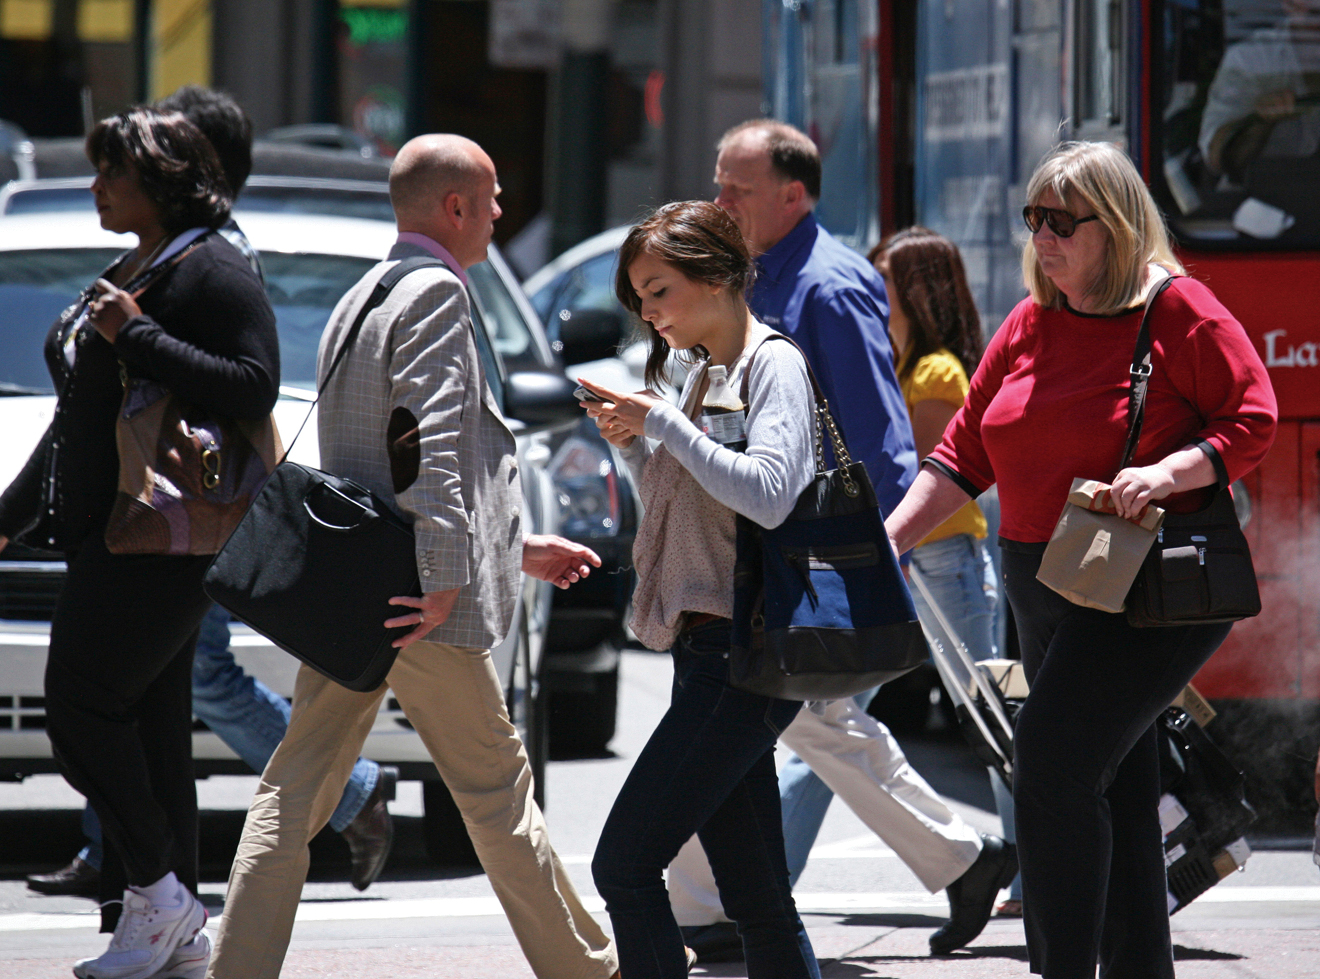
\includegraphics[height=3.9cm]{figures_introduction/pedestrian}}
	\subcaptionbox{\footnotesize Lighting Variation\label{fig:difficult_b}}{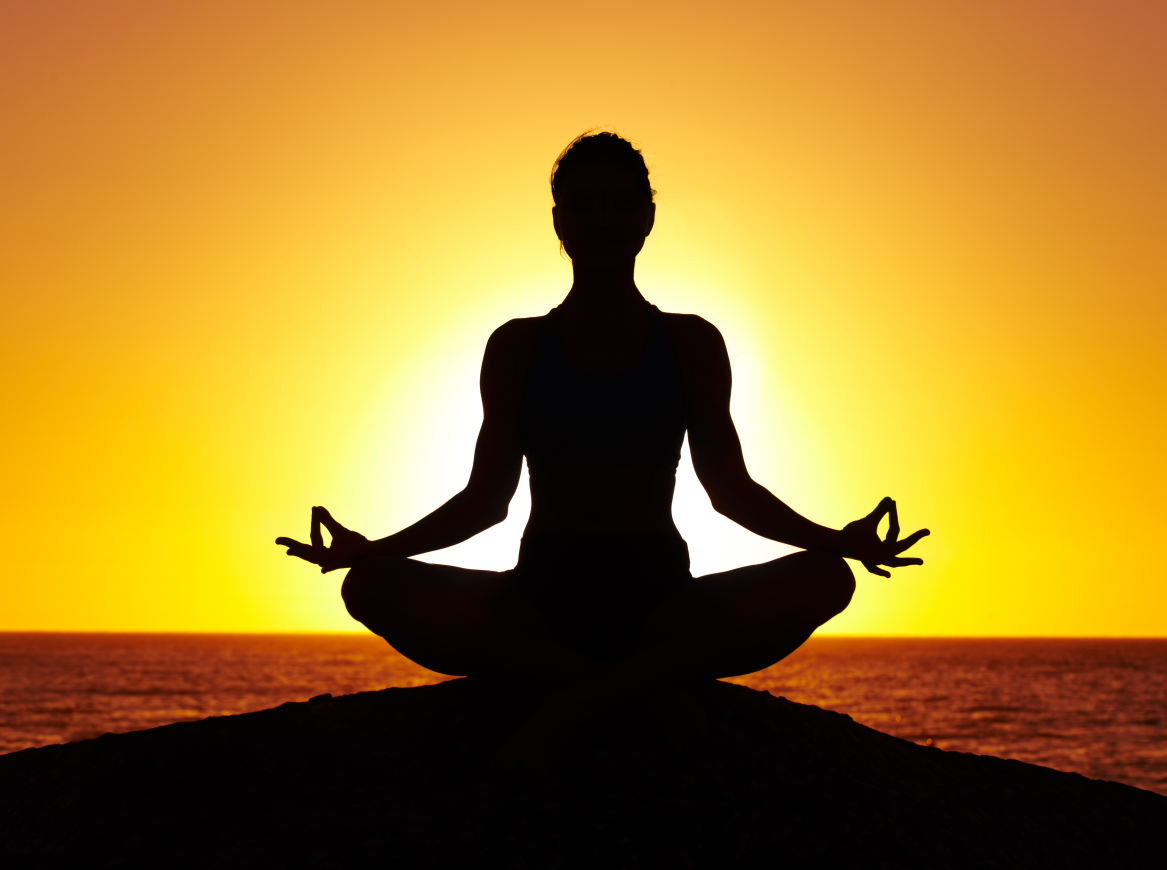
\includegraphics[trim=1.7cm 1.0cm 1.5cm 0.5cm, clip=true, height=3.9cm]{figures_introduction/yoga-pose}}
	\subcaptionbox{\footnotesize Self Occlusion\label{fig:difficult_c}}{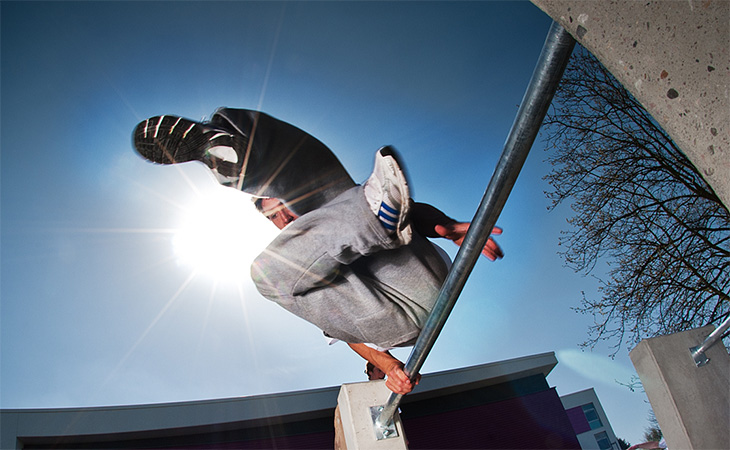
\includegraphics[trim=3.0cm 0.0cm 6.5cm 2.0cm, clip=true, height=3.9cm]{figures_introduction/x-move_parkour_.jpg}}
        \caption{Difficult Samples for Human Body Pose Recognition}
        \label{fig:difficult}
\end{figure}

Human body localization is complicated and difficult for numerous reasons, and some difficult examples are shown in Figure~\ref{fig:difficult}. As with many computer vision applications, the high dimensional nature of the image input makes inferring the low-dimensional pose representation difficult since the input dimensionality cannot be easily enumerated. However, unlike many classic computer vision tasks, human body tracking also involves localizing body parts that undergo large amounts of deformation and exhibit wide variation in both body-shape and appearance. Deformation increases the intrinsic input dimensionality of the space of possible poses and furthermore leads to occlusion, which means that pose inference must be performed with potentially missing data. Appearance variation can be the result of clothing, lighting variation or the subjects age or gender; therefore any inference solution must learn invariance in order to provide a stable estimate of pose under such wildly varying conditions. Lastly, large and comprehensive datasets exist for image classification tasks~\cite{deng2009imagenet}, however human-body pose datasets are many orders of magnitude smaller~\cite{modec,andriluka14cvpr,Johnson10}. The lack of a comprehensive standard dataset has traditionally made training robust discriminative architectures difficult as such networks are prone to over-training when the training set sizes are limited.

Despite these significant challenges, this work will present a framework for human body pose localization that offers a significant improvement over existing traditional architectures. The basis for all the tracking solutions presented in this thesis is the use of Convolutional Networks (ConvNets), which have seen a recent surge in success and popularity due to advances in Graphics Processing Unit (GPU) hardware as well as new and improved techniques for training them. ConvNets are biologically inspired variants of multi-layered perceptrons, which exploit spatial correlation in natural images by extracting features generated by localized convolution kernels. In the context of object detection, the use of fully convolutional networks result in trained detectors which are invariant to translation, and this work makes heavy use of this feature for the architectures presented in Parts \ref{part:two}, \ref{part:three} and \ref{part:four}. A full-review of ConvNets - specifically their formulation and training via the Back-Propagation algorithm - is outside the scope of this thesis and interested readers should refer to \cite{reading_list} for an overview of seminal literature.

ConvNets have been used successfully to solve many difficult machine learning problems: image classification~\cite{pedestrianCVPR13, overfeatSermanet, ImageNet_NIPS2012_0534, googlenet}, scene understanding~\cite{Farabet}, video analysis~\cite{KarpathyCVPR14} and natural language processing~\cite{ilya_sequence,cho_emnlp_2014}. Likewise, they have recently out-performed all existing models on the task of hand-pose recognition~\cite{tompsonTOG14} using an depth camera source, and monocular human-body pose recognition using an RGB camera~\cite{tompsonnips2014, arjunaccv2014, jainiclr2014, deeppose, chennips2014, tompson_efficient}. In this work, we will present our results for the current state-of-the-art models (at time of writing) for human body and hand pose recognition.

\subsection*{Thesis Outline}

This thesis will explore solutions to two difficult computer vision problems related to the localization of humans in images: 1) monocular hand-pose recognition from depth images and 2) monocular full body-pose recognition from RGB images. This exploration will cover four primary publications \cite{tompsonTOG14}, \cite{tompsonnips2014}, \cite{arjunaccv2014}, \cite{tompson_efficient} in Parts \ref{part:one}, \ref{part:two}, \ref{part:three} and \ref{part:four} respectively. Within each part, the first section will define the specific problem and present an overview of the architecture. The second section will present the model and any algorithmic details necessary to repeat experiments. Then the final solution will present experimental results, compare our work with previous state-of-the-art and describe any limitations.

\subsection*{Summary of Contributions}

The following is a summary of the major contributions of this thesis:

\begin{itemize}

\item In Part~\ref{part:one} we describe a novel pipeline for both offline ground truth dataset creation, as well as real-time pose-detection of human hands in depth video. While Neural Networks have been used for pose detection of a limited set of discrete hand gestures (for instance discriminating between a closed fist and an open palm)~\cite{nagi,nowlan}, to our knowledge this is the first work that has attempted to use such networks to perform dense feature extraction of human hands in order to infer continuous pose.

\item In Part~\ref{part:two} we describe a novel ConvNet architecture which combines a traditional sliding-window based part detector with a Graphical Model. We describe a graphical model formulation which is inspired by standard MRF belief propagation, which can be trained jointly with a standard deep-learning architecture to improve detection performance. At the time of writing, this model is the state-of-the-art model for the FLIC~\cite{modec}, LSP~\cite{Johnson10} and MPII~\cite{andriluka14cvpr} datasets.

\item In Part~\ref{part:three} we show that simple motion features can be used to significantly improve the performance of traditional ConvNet architectures. To our knowledge, this was the first work to empirically examine the impact of multi-frame inputs to ConvNets in the application of pose detection.

\item In Part~\ref{part:four} we examine the issue of localization accuracy degradation in ConvNet architecture due to spatial-pooling layers. We present a novel cascaded architecture, that makes use of shared features, in order to improve localization accuracy while maintaining runtime performance. We are the first to show that a ConvNet trained to infer the 2D pose of humans in images is able to be competitive with - and in some cases out-perform - humans trained on the same task.

\end{itemize}
\chapter{Related Work}
\label{chapter:related_work}
\begin{table} 
\begin{center} 
\begin{tabular}{|c||c|c|c|c|}
\hline
\emph{Algorithm} & \emph{Manifold Model} & \emph{Encode} & \emph{Decode} & \emph{Relate Enc. \& Dec.}\\
%\thickhline
\hline \hline 
\cellcolor{red}PCA & Linear &\checkmark & \checkmark & $W_D = W_E ^T$\\
\hline
\cellcolor{red}ICA & Linear &\checkmark & \checkmark & $W_D = W_E ^T$\\
\hline
\cellcolor{yellow}Sparse Coding & Local Linear &\checkmark & \checkmark & Separate \\
\hline 
\cellcolor{yellow}PSD \& LISTA & Local Linear &\checkmark & \checkmark & Separate\\
\hline
\cellcolor{lightblue}DrLIM & Nonlinear & \checkmark & X & Enc. Only\\
\hline
\cellcolor{lightblue}Chapter \ref{chapter:slow} & Nonlinear & \checkmark & X & Enc. Only\\
\hline
\cellcolor{lightblue}Chapter \ref{chapter:linear} & Nonlinear & \checkmark & \checkmark & Separate\\
\hline
Adversarial Networks & Nonlinear & X & \checkmark & Dec. Only \\
\hline 
\cellcolor{green}Auto-Encoders & Nonlinear & \checkmark & \checkmark & Separate \\
\hline 
\end{tabular} \\
\vspace{0.25cm} \hspace{0.25cm}  
\begin{tabular}{|c|}
\hline 
\emph{Model Objective/Prior}\\  
\hline \hline
\cellcolor{red} De-correlation/Independence  \\
\hline
\cellcolor{yellow} Sparsity \\
\hline
\cellcolor{lightblue} Metric Learning/Geometric Prior  \\
\hline
\cellcolor{green} All of the Above \\
\hline
None \\
\hline
\end{tabular}
\end{center}
\caption{Summary of unsupervised feature learning algorithms and their properties} 
\label{tbl:models} 
\end{table} 

Unsupervised feature learning arguably dates back to the invention of Principal
Component Analysis (PCA) in 1901 by Karl Pearson \cite{PCA}. As mentioned in
Chapter \ref{chapter:introduction}, feature learning algorithms model
intrinsically low dimensional data embedded in a high dimensional ambient
space. These models can usually be decomposed into two parts: a mapping from
the input space to the feature space, called encoding, and mapping the feature
space back to the input space, called decoding. If the encoding or decoding
processes have corresponding functional forms, they are referred to as the
``encoder'' and ``decoder'', respectively.  From the natural image manifold
perspective, ideal encodings map the extrinsic coordinates (i.e. pixel values)
to intrinsic manifold coordinates. It is hoped that these intrinsic coordinates
correspond to physical attributes of the natural world, such as the presence of
certain objects in the scene, their properties, etc \cite{nair2008,capsules}.
Unsupervised feature learning models are mainly distinguished by: i-the
geometrical prior they assume about the data manifold, ii-whether they learn an
encoder, decoder, or both. For example, Principal Component Analysis assumes
that the data is concentrated around a hyper-plane, i.e. it assumes a globally
linear data manifold model. The PCA encoder is a matrix operator, $W_e$, as is
the decoder $W_d=W_e^T$.  Obtaining ``invariant'' representations has been a
major driving force in feature learning, driven mainly by recognition and
classification problems.  Invariant features imply that the encoding process is
necessarily a many-to-one mapping. This means that the decoding process must
involve some random selection among the possible inputs that produced the code,
usually  by sampling from a distribution. Models that include a decoder are
called ``generative models'' in the literature. 

Table \ref{tbl:models} summarizes key aspects of several well-known feature
learning models, as well as the new models which will be introduced in Chapters
\ref{chapter:slow} and \ref{chapter:linear}. The first column lists the name of
the model, the color indicates the type of objective each model tries to
optimize.  These are summarized in the table below. For example, one version of
PCA finds maximally decorrelated linear components. The ``manifold model''
column indicates the geometric prior each model assumes about the data
manifold. The next two columns indicate whether each model learns an encoder
and/or decoder.  Finally, the last column summarizes the relationship enforced
between the encoder and decoder. For example in PCA the encoder and decoder are
related by the transpose operator. This chapter will review the algorithms in
Table \ref{tbl:models}, placing emphasis on the precursors of the algorithms
presented in Chapters \ref{chapter:slow} and \ref{chapter:linear}. The
algorithms will be presented as various models of the data manifold.

\section{Principal and Independent Component Analysis} 

\begin{figure} 
\centering
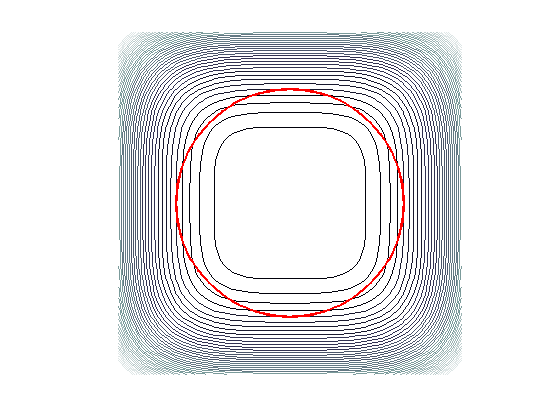
\includegraphics[scale=0.4]{./figures/related_work/ICA.png} 
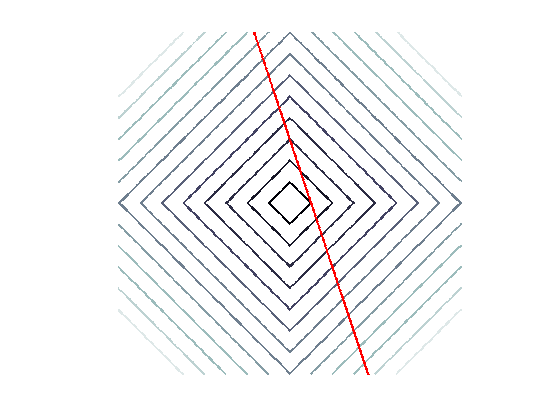
\includegraphics[scale=0.4]{./figures/related_work/L1.png} 
\caption{Left: visualization of the optimization problem used to solve for independent representations. Right: visualization of the optimization problem used to solve for sparse representations.} 
\label{fig:ICA_lasso} 
\end{figure}  

Principal Component Analysis (PCA) and Independent Component Analysis (ICA) are
the most well know linear manifold models \cite{ICA}. Both assume that the
observed high dimensional data $x$ are generated from some low dimensional
latent variables $z$ via a linear operator $A$, that is $x=Az$. Assuming that
the data is zero mean, PCA implicitly makes the assumption that the latent
variables correspond to directions with the largest variance \cite{PCA}.  These
components can be obtained from the Eigen decomposition of the covariance
matrix.  ICA however searches for linearly independent components, formulating
the definition of independence using the central limit theorem. Although the
detailed derivation of ICA will not be presented here, we will mention that it
leads to a fourth order moment (kurtosis) maximization problem subject to a
second order moment (variance) constraint. This optimization problem is
visualized as the left plot of Figure \ref{fig:ICA_lasso}. The blue curves
represent the level sets of the kurtosis objective, and the red curve
represents the unit variance constraint. The next section will establish a 
remarkable connection between ICA and sparse inference.  

\section{Sparse Representations} 
Sparse inference refers to the problem of finding the coefficients $z$ which
reconstruct the input $x$ as a sparse linear combination of some basis elements
contained an over-complete dictionary $W_d$. Sparsity is measured by the number
of non-zero coefficients; the higher the sparsity the fewer non-zero
coefficients in $z$ used to represent $x$.  
The sparse inference problem can be stated formally as: 

\begin{equation} 
min \|z\|_0 \mbox{ subject to } x = W_dz 
\end{equation} 

In general, this is an intractable combinatorial problem. A now famous
breakthrough showed that exact sparse solutions can be obtained, under certain
conditions, by replacing the $L_0$ norm with an $L_1$ norm \cite{candes2006}.
This optimization problem is depicted on the right side of Figure
\ref{fig:ICA_lasso}.  The level sets of the $L_1$ norm are shown in blue and
the linear constraint is shown in red. The minimum occur on the $x$-axis, with
$y=0$ implying that the solution is indeed sparse. Remarkably, the solution to
the ICA problem (left side of Figure \ref{fig:ICA_Lasso}) is also sparse though the
objective was explicitly derived with sparsity in mind.    

Relaxing the constraint, this problem can be written as an unconstrained loss
functional called the lasso (also basis pursuit de-noising) \cite{BP}:  

\begin{equation} 
L_{lasso} = \frac{1}{2}\|x-W_dz\| + \alpha |z|_1
\end{equation} 


\section{Metric Learning}

\section{Auto-Encoders and Energy Based Learning} 
 
 
\chapter{Saturating Auto-Encoders}
\label{chapter:SATAE}
\section{Introduction} 
This Chapter introduces a new latent state regularization method for auto-encoders. 
We show that the saturation regularizer explicitly limits the auto-encoder's capacity to
reconstruct inputs which are not near the data manifold. Connections are established with 
other auto-encoder regularization methods, as well as with the partition function in 
probabilistic models. 

When minimizing reconstruction loss alone, the standard auto-encoder
does not typically learn any meaningful hidden representation of the data. Well
known theoretical and experimental results show that a linear auto-encoder with
trainable encoding and decoding matrices, $W^e$ and $W^d$ respectively, learns
the identity function if $W^e$ and $W^d$ are full rank or over-complete. The
linear auto-encoder learns the principle variance directions (PCA) if $W^e$ and
$W^d$ are rank deficient \cite{DHS}. It has been observed that other
representations can be obtained by regularizing the latent representation. This
approach is exemplified by the Contractive and Sparse Auto-Encoders \cite{CAE}
\cite{SAE1} \cite{SAE2}. Intuitively, an auto-encoder with limited capacity
will focus its resources on reconstructing portions of the input space in which
data samples occur most frequently. From an energy based perspective,
auto-encoders achieve low reconstruction cost in portions of the input space
with high data density (recently, \cite{bengio_new} has examined this
perspective in depth). If the data occupies some low dimensional manifold in
the higher dimensional input space then minimizing reconstruction error
achieves low energy on this manifold. Useful latent state regularizers raise
the energy of points that do not lie on the manifold, thus playing an analogous
role to minimizing the partition function in maximum likelihood models. In this
work we introduce a new type of regularizer that does this explicitly for
auto-encoders with a non-linearity that contains at least one flat (zero
gradient) region. We show examples where this regularizer and the choice of
nonlinearity determine the feature set that is learned by the auto-encoder.      

\section{Latent State Regularization}  Several auto-encoder variants which
regularize their latent states have been proposed, they include the sparse
auto-encoder and the contractive auto-encoder\cite{SAE1}\cite{SAE2}\cite{CAE}.
The sparse auto-encoder includes an over-complete basis in the encoder and
imposes a sparsity inducing (usually $L_1$) penalty on the hidden activations.
This penalty prevents the auto-encoder from learning to reconstruct all
possible points in the input space and focuses the expressive power of the
auto-encoder on representing the data-manifold. Similarly, the contractive
auto-encoder avoids trivial solutions by introducing an auxiliary penalty which
measures the square  Frobenius norm of the Jacobian of the latent
representation with respect to the inputs. This encourages a constant latent
representation except around training samples where it is counteracted by the
reconstruction term. It has been noted in \cite{CAE} that these two approaches
are strongly related. The contractive auto-encoder explicitly encourages small
entries in the Jacobian, whereas the sparse auto-encoder is encouraged to
produce mostly zero (sparse) activations which can be designed to correspond to
mostly flat regions of the nonlinearity, thus also yielding small entries in
the Jacobian.

\subsection{Saturating Auto-Encoder through Complementary Nonlinearities}
Our goal is to introduce a simple new regularizer which explicitly raises
reconstruction error for inputs not near the data manifold. Consider activation
functions with at least one flat region; these include shrink, rectified
linear, and saturated linear (Figure~\ref{fig:nonlin}). Auto-encoders with such
nonlinearities lose their ability to accurately reconstruct inputs which
produce activations in the zero-gradient regions of their activation functions.
Let us denote the auto-encoding function $x_r = G(x,W)$, $x$ being the input,
$W$ the trainable parameters in the auto-encoder, and $x_r$ the reconstruction.
One can define an energy surface through the reconstruction error: \[ E_W(x) =
||x-G(x,W)||^2 \] Let's imagine that $G$ has been trained to produce a low
reconstruction error at a particular data point $x^*$. If $G$ is constant when
$x$ varies along a particular direction $v$, then the energy will grow
quadratically along that particular direction as $x$ moves away from $x^*$. If
$G$ is trained to produce low reconstruction errors on a set of samples while
being subject to a regularizer that tries to make it constant in as many
directions as possible, then the reconstruction energy will act as a {\em
contrast function} that will take low values around areas of high data density
and larger values everywhere else (similarly to a negative log likelihood
function for a density estimator).

The proposed auto-encoder is a simple implementation of this idea.  Using the
notation $W =\{W^e,B^e,W^d,B^d\}$, the auto-encoder function is defined as \[
G(x,W) = W^d F(W^e x+B^e) + B^d \] where $W^e$, $B^e$, $W^d$, and $B^d$ are the
encoding matrix, encoding bias, decoding matrix, and decoding bias,
respectively, and $F$ is the vector function that applies the scalar function
$f$ to each of its components. $f$ will be designed to have "flat spots", i.e.
regions where the derivative is zero (also referred to as the saturation
region).

The loss function minimized by training is the sum of the reconstruction energy
$E_W(x)=||x-G(x,W)||^2$ and a term that pushes the components of $W^e x + B^e$
towards the flat spots of $f$. This is performed through the use of a {\em
complementary function} $f_c$, associated with the non-linearity $f(z)$. The
basic idea is to design $f_c(z)$ so that its value corresponds to the distance
of $z$ to one of the flat spots of $f(z)$. Minimizing $f_c(z)$ will push $z$
towards the flat spots of $f(z)$. With this in mind, we introduce a penalty of
the form $f_c(\sum_{j=1}^d W^e_{ij}x_j + b^e_i)$ which encourages the argument
to be in the saturation regime of the activation function ($f$). We refer to
auto-encoders which include this regularizer as Saturating Auto-Encoders
(SATAEs). For activation functions with zero-gradient regime(s) the
complementary nonlinearity ($f_c$) can be defined as the distance to the
nearest saturation region. Specifically, let $S = \{z \mid  f'(z) = 0\}$ then
we define $f_c(z)$ as: 

\begin{equation} f_c(z) = \inf_ {z' \in S} |z-z'|.   \end{equation}   

\begin{figure} \centering 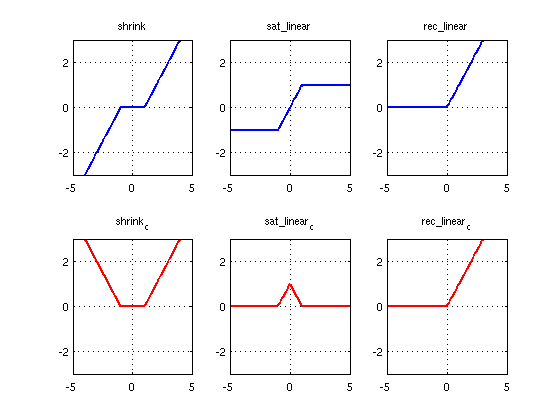
\includegraphics[scale=0.6]{./figures/SATAE/compliments.png}
\caption{Three nonlinearities (top) with their associated complementary
regularization functions(bottom).}  \label{fig:nonlin} \end{figure} 

\noindent Figure 1 shows three activation functions and their associated
complementary nonlinearities. The complete loss to be minimized by a SATAE with
nonlinearity $f$ is: 

\begin{equation} L = \sum_{x \in D} \frac{1}{2} \|x-\left(W^d F(W^e
x+B^e)+B^d\right)\|^2 + \alpha \sum_{i=1}^{d_h}f_c(W^e_i x + b^e_i),
\end{equation}    

\noindent where $d_h$ denotes the number of hidden units. The hyper-parameter
$\alpha$ regulates the trade-off between reconstruction and saturation.  

\section{Effect of the Saturation Regularizer} We will examine the effect of
the saturation regularizer on auto-encoders with a variety of activation
functions. It will be shown that the choice of activation function is a
significant factor in determining the type of basis the SATAE learns. First, we
will present results on toy data in two dimensions followed by results on
higher dimensional image data.

\subsection{Visualizing the Energy Landscape}  Given a trained auto-encoder the
reconstruction error can be evaluated for a given input $x$. For
low-dimensional spaces ($\mathbb{R}^n$, where $n \leq 3$) we can evaluate the
reconstruction error on a regular grid in order to visualize the portions of
the space which are well represented by the auto-encoder. More specifically we
can compute $E(x) = \frac{1}{2} \|x - x_r \|^2$ for all $x$ within some bounded
region of the input space. Ideally, the reconstruction energy will be low for
all $x$ which are in the training set and high elsewhere.
Figures~\ref{fig:toyshrink} and~\ref{fig:toysatlinear} depict the resulting
reconstruction energy for inputs $x \in \mathbb{R}^2$, and  $-1 \leq x_i \leq
1$. Black corresponds to low reconstruction energy. The training data consists
of a one dimensional manifold shown overlain in yellow.
Figure~\ref{fig:toyshrink} shows a toy example for a SATAE which uses ten basis
vectors and a shrink activation function. Note that adding the saturation
regularizer decreases the volume of the space which is well reconstructed,
however good reconstruction is maintained on or near the training data
manifold. The auto-encoder in Figure~\ref{fig:toysatlinear} contains two
encoding basis vectors (red), two decoding basis vectors (green), and uses a
saturated-linear activation function. The encoding and decoding bases are
unconstrained. The unregularized auto-encoder learns an orthogonal basis with a
random orientation. The region of the space which is well reconstructed
corresponds to the outer product of the linear regions of two activation
functions; beyond that the error increases quadratically with the distance.
Including the saturation regularizer induces the auto-encoder basis to align
with the data and to operate in the saturation regime at the extreme points of
the training data, which limits the space which is well reconstructed. Note
that because the encoding and decoding weights are separate and unrestricted,
the encoding weights were scaled up to effectively reduce the width of the
linear regime of the nonlinearity. 

\subsection{SATAE-shrink} Consider a SATAE with a shrink activation function
and shrink parameter $\lambda$. The corresponding complementary nonlinearity,
derived using Equation 1 is given by: \begin{equation} \nonumber shrink_c(x) =
\begin{cases} abs(x), \text{ } |x| > \lambda\\ 0, \text{ elsewhere}
\end{cases}.  \end{equation} 

\begin{figure} \centering 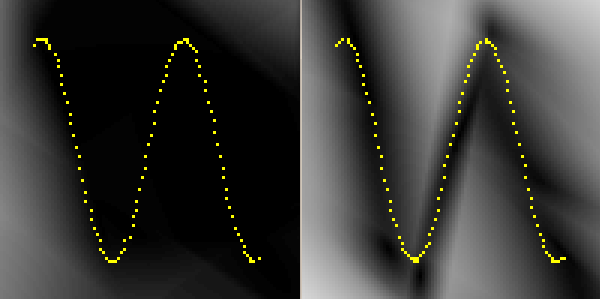
\includegraphics[scale=0.25]{./figures/SATAE/toy_shrink.png}
\caption{Energy surfaces for unregularized (left), and regularized (right)
solutions obtained on SATAE-shrink and 10 basis vectors. Black corresponds to
low reconstruction energy. Training points lie on a one-dimensional manifold
shown in yellow.}  \label{fig:toyshrink} \end{figure} 

\begin{figure} \centering
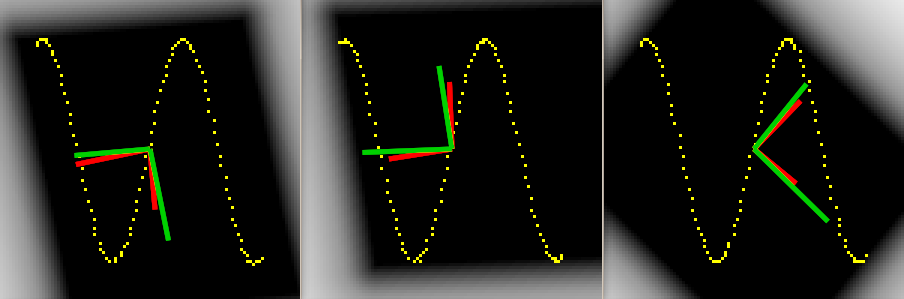
\includegraphics[scale=0.25]{./figures/SATAE/toy_sat_linear_noreg.png}
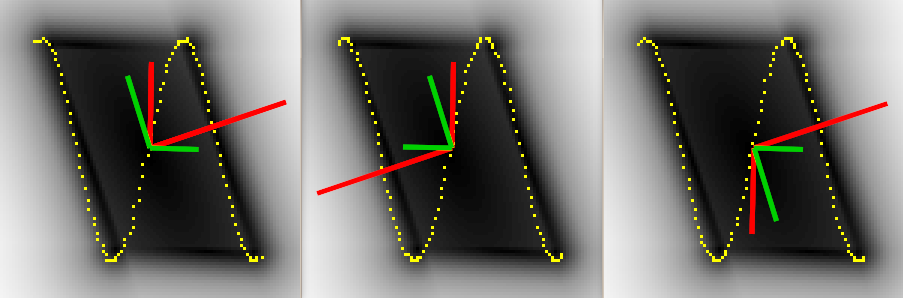
\includegraphics[scale=0.25]{./figures/SATAE/toy_sat_linear_reg.png} \caption{SATAE-SL toy
example with two basis elements. Top Row: three randomly initialized solutions
obtained with no regularization. Bottom Row: three randomly initialized
solutions obtained with regularization.}  \label{fig:toysatlinear} \end{figure} 

Note that $shrink_c(W^e x + b^e) =  abs(shrink(W^e x + b^e))$, which
corresponds to an $L_1$ penalty on the activations. Thus this SATAE is
equivalent to a sparse auto-encoder with a shrink activation function. Given
the equivalence to the sparse auto-encoder we anticipate the same scale
ambiguity which occurs with $L_1$ regularization. This ambiguity can be avoided
by normalizing the decoder weights to unit norm. It is expected that the
SATAE-shrink will learn similar features to those obtained with a sparse
auto-encoder, and indeed this is what we observe. Figure~\ref{fig:results}(c)
shows the decoder filters learned by an auto-encoder with shrink nonlinearity
trained on gray-scale natural image patches. One can recognize the expected
Gabor-like features when the saturation penalty is activated. When trained on
the binary MNIST dataset the learned basis is comprised of portions of digits
and strokes. Nearly identical results are obtained with a SATAE which uses a
rectified-linear activation function. This is because a rectified-linear
function with an encoding bias behaves as a positive only shrink function,
similarly the complementary function is equivalent to a positive only $L_1$
penalty on the activations.          

\newcommand\x{2.5cm}
\newcommand\y{8cm} 

\afterpage{
%\clearpage
\thispagestyle{empty}
\begin{figure} 
\centering \begin{subfigure}[b]{0.225\textwidth} \centering
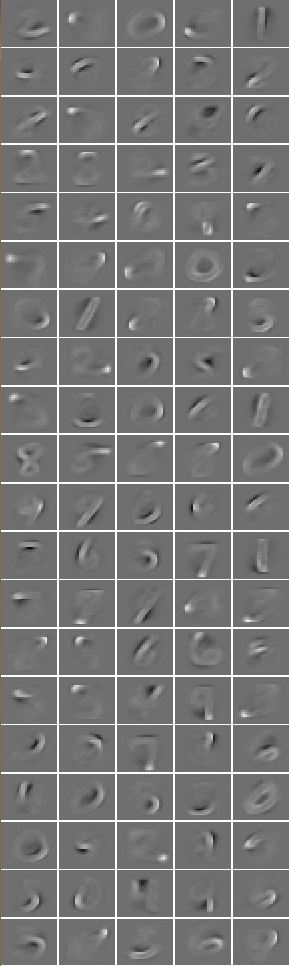
\includegraphics[width=\x, height=\y]{./figures/SATAE/strokes_full.png} \caption{}
\end{subfigure} \begin{subfigure}[b]{0.225\textwidth} \centering
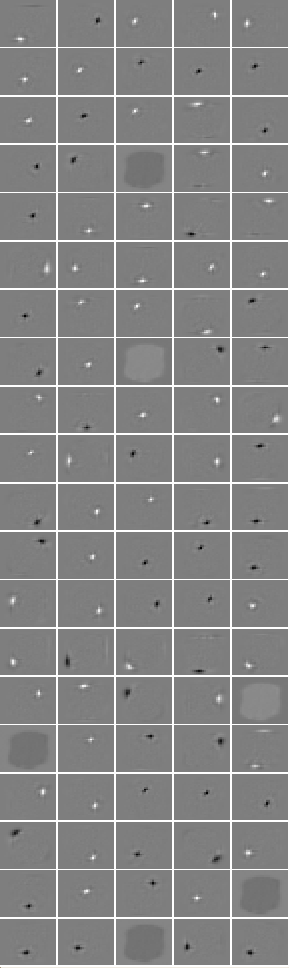
\includegraphics[width=\x, height=\y]{./figures/SATAE/MNIST_sat_linear_full.png}
\caption{} \end{subfigure} \begin{subfigure}[b]{0.2\textwidth} \centering
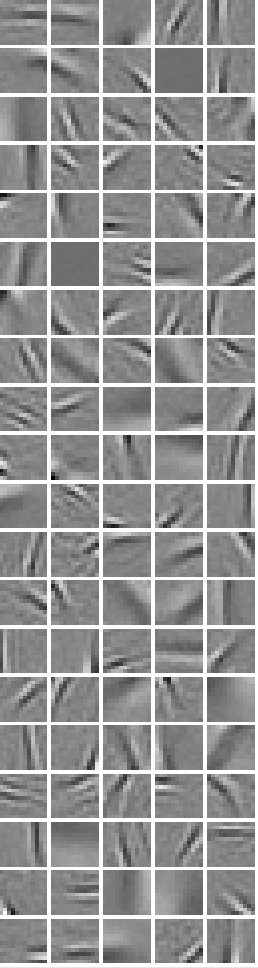
\includegraphics[width=\x, height=\y]{./figures/SATAE/gabors_full.png} \caption{}
\end{subfigure} \begin{subfigure}[b]{0.2\textwidth} \centering
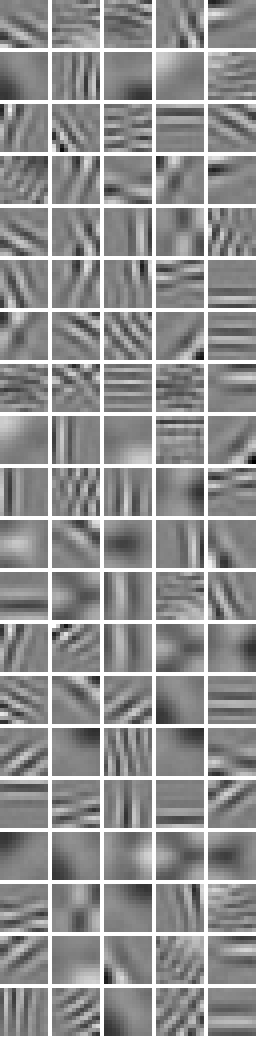
\includegraphics[width=\x, height=\y]{./figures/SATAE/patches_sat_linear_full.png}
\caption{} \end{subfigure} \\ \begin{subfigure}[b]{0.225\textwidth} \centering
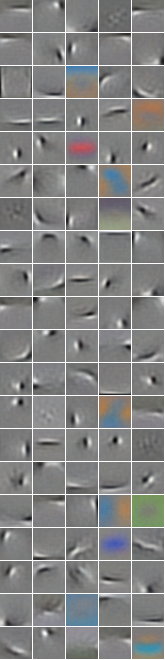
\includegraphics[width=\x, height=\y]{./figures/SATAE/CIFAR_shrink01.png} \caption{}
\end{subfigure} \begin{subfigure}[b]{0.225\textwidth} \centering
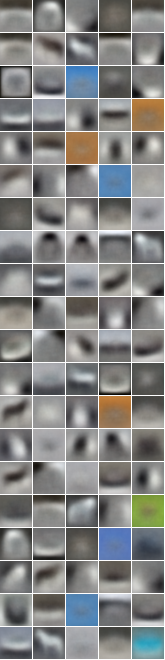
\includegraphics[width=\x, height=\y]{./figures/SATAE/CIFAR_shrink05.png} \caption{}
\end{subfigure} \begin{subfigure}[b]{0.2\textwidth} \centering
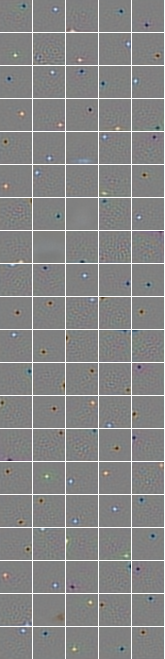
\includegraphics[width=\x, height=\y]{./figures/SATAE/CIFAR_sat_linear300_1.png}
\caption{} \end{subfigure} \begin{subfigure}[b]{0.2\textwidth} \centering
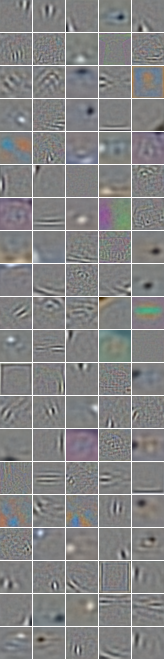
\includegraphics[width=\x, height=\y]{./figures/SATAE/CIFAR_sat_linear300_6.png}
\caption{} \end{subfigure} \caption{\small Basis elements learned by the SATAE using
different nonlinearities on: 28x28 binary MNIST digits, 12x12 gray scale
natural image patches, and CIFAR-10. (a) SATAE-shrink trained on MNIST, (b)
SATAE-saturated-linear trained on MNIST, (c) SATAE-shrink trained on natural
image patches, (d) SATAE-saturated-linear trained on natural image patches,
(e)-(f) SATAE-shrink trained on CIFAR-10 with $\alpha=0.1$ and $\alpha=0.5$,
respectively, (g)-(h) SATAE-SL trained on CIFAR-10 with $\alpha=0.1$ and
$\alpha=0.6$, respectively.  } \label{fig:results} \end{figure}
\clearpage} 

\begin{figure} \centering 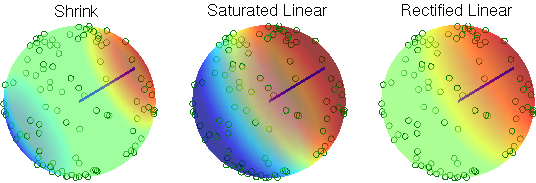
\includegraphics[scale=0.5]{./figures/SATAE/viz_nonlin.png}
\caption{Geometric visualization of non-linearities}
\end{figure} 


\begin{figure} \centering \begin{subfigure}[b]{0.15\textwidth} \centering
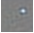
\includegraphics[scale=2]{./figures/SATAE/1.png}\\ 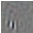
\includegraphics[scale=2]{./figures/SATAE/horse1.png} 
        %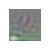
\includegraphics[scale=2]{.//objects/red/0.png} \\
        %\caption{$\alpha=0$}
    \end{subfigure} \begin{subfigure}[b]{0.15\textwidth} \centering
    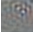
\includegraphics[scale=2]{./figures/SATAE/2.png} \\
    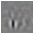
\includegraphics[scale=2]{./figures/SATAE/horse2.png} 
        %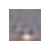
\includegraphics[scale=2]{.//objects/red/1.png} \\
        %\caption{$\alpha=0.1$}
    \end{subfigure} \begin{subfigure}[b]{0.15\textwidth} \centering
    
\includegraphics[scale=2]{./figures/SATAE/3.png}\\
    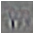
\includegraphics[scale=2]{./figures/SATAE/horse3.png} 
        %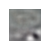
\includegraphics[scale=2]{.//objects/red/2.png} \\
		
        %\caption{$\alpha=0.2$}
    \end{subfigure} \begin{subfigure}[b]{0.15\textwidth} \centering
    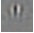
\includegraphics[scale=2]{./figures/SATAE/4.png} \\
    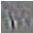
\includegraphics[scale=2]{./figures/SATAE/horse4.png} 
        %
\includegraphics[scale=2]{.//objects/red/3.png} \\
        %\caption{$\alpha=0.5$}
    \end{subfigure} \begin{subfigure}[b]{0.15\textwidth} \centering
    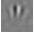
\includegraphics[scale=2]{./figures/SATAE/5.png} 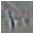
\includegraphics[scale=2]{./figures/SATAE/horse5.png}
    \\
        %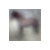
\includegraphics[scale=2]{./objects/red/4.png} \\
		
        %\caption{$\alpha=1$} 
    \end{subfigure} \caption{Evolution of two filters with increasing
    saturation regularization for a SATAE-SL trained on CIFAR-10. Filters
    corresponding to larger values of $\alpha$ were initialized using the
    filter corresponding to the previous $\alpha$. The regularization parameter
    was varied from 0.1 to 0.5 (left to right) in the top five images and 0.5
    to 1 in the bottom five } \label{fig:horse} \end{figure} 

\subsection{SATAE-saturated-linear} Unlike the SATAE-shrink, which tries to
compress the data by minimizing the number of active elements; the SATAE
saturated-linear (SATAE-SL) tries to compress the data by encouraging the
latent code to be as close to binary as possible. Without a saturation penalty
this auto-encoder learns to encode small groups of neighboring pixels. More
precisely, the auto-encoder learns the identity function on all datasets. An
example of such a basis is shown in Figure \ref{fig:results}(b). With this
basis the auto-encoder can perfectly reconstruct any input by producing small
activations which stay within the linear region of the nonlinearity.
Introducing the saturation penalty does not have any effect when training on
binary MNIST. This is because the scaled identity basis is a global minimizer
of Equation 2 for the SATAE-SL on any binary dataset. Such a basis can
perfectly reconstruct any binary input while operating exclusively in the
saturated regions of the activation function, thus incurring no saturation
penalty. On the other hand, introducing the saturation penalty when training on
natural image patches induces the SATAE-SL to learn a more varied basis (Figure
\ref{fig:results}(d)). 

\subsection{Experiments on CIFAR-10} SATAE auto-encoders with 100 and 300 basis
elements were trained on the CIFAR-10 dataset, which contains small color
images of objects from ten categories. In all of our experiments the
auto-encoders were trained by progressively increasing the saturation penalty
(details are provided in the next section). This allowed us to visually track
the effect of the saturation penalty on individual basis elements. Figure
\ref{fig:results}(e)-(f) shows the basis learned by SATAE-shrink with small and
large saturation penalty, respectively. Increasing the saturation penalty has
the expected effect of reducing the number of nonzero activations. As the
saturation penalty increases, active basis elements become responsible for
reconstructing a larger portion of the input. This induces the basis elements
to become less spatially localized. This effect can be seen by comparing
corresponding filters in Figure \ref{fig:results}(e) and (f). Figures
\ref{fig:results}(g)-(h)  show the basis elements learned by SATAE-SL with
small and large saturation penalty, respectively. The basis learned by SATAE-SL
with a small saturation penalty resembles the identity basis, as expected (see
previous subsection). Once the saturation penalty is increased small
activations become more heavily penalized. To increase their activations the
encoding basis elements may increase in magnitude or align themselves with the
input. However, if the encoding and decoding weights are tied (or fixed in
magnitude) then reconstruction error would increase if the weights were merely
scaled up. Thus the basis elements are forced to align with the data in a way
that also facilitates reconstruction. This effect is illustrated in Figure
\ref{fig:horse} where filters corresponding to progressively larger values of
the regularization parameter are shown. The top half of the figure shows how an
element from the identity basis ($\alpha=0.1$) transforms to a localized edge
($\alpha=0.5$). The bottom half of the figure shows how a localized edge
($\alpha=0.5$) progressively transforms to a template of a horse ($\alpha=1$).

\section{Experimental Details} Because the regularizer explicitly encourages
activations in the zero gradient regime of the nonlinearity, many encoder basis
elements would not be updated via back-propagation through the nonlinearity if
the saturation penalty were large. In order to allow the basis elements to
deviate from their initial random states we found it necessary to progressively
increase the saturation penalty. In our experiments the weights obtained at a
minimum of Equation 2 for a smaller value of $\alpha$ were used to initialize
the optimization for a larger value of $\alpha$. Typically, the optimization
began with $\alpha=0$ and was progressively increased to $\alpha=1$ in steps of
$0.1$. The auto-encoder was trained for 30 epochs at each value of $\alpha$.
This approach also allowed us to track the evolution of basis elements as a
function of $\alpha$ (Figure \ref{fig:horse}). In all experiments data samples
were normalized by subtracting the mean and dividing by the standard deviation
of the dataset. The auto-encoders used to obtain the results shown in Figure
\ref{fig:results} (a),(c)-(f) used 100 basis elements, others used 300 basis
elements. Increasing the number of elements in the basis did not have a strong
qualitative effect except to make the features represented by the basis more
localized. The decoder basis elements of the SATAEs with shrink and
rectified-linear nonlinearities were reprojected to the unit sphere after every
10 stochastic gradient updates. The SATAEs which used saturated-linear
activation function were trained with tied weights.  All results presented were
obtained using stochastic gradient descent with a constant learning rate of
0.05.

\section{Discussion}

In this work we have introduced a general and conceptually simple latent state
regularizer. It was demonstrated that a variety of feature sets can be obtained
using a single framework. The utility of these features depend on the
application. In this section we extend the definition of the saturation
regularizer to include functions without a zero-gradient region. The
relationship of SATAEs with other regularized auto-encoders will be discussed.
We conclude with a discussion on future work.   

\subsection{Extension to Differentiable Functions} We would like to extend the
saturation penalty definition (Equation 1) to differentiable functions without
a zero-gradient region. An appealing first guess for the complimentary function
is some positive function of the first derivative, $f_c(x) = |f'(x)|$ for
instance. This may be an appropriate choice for monotonic activation functions
which have their lowest gradient regions at the extrema (e.g. sigmoids).
However some activation functions may contain regions of small or zero gradient
which have negligible extent, at the extrema for instance. We would like our
definition of the complimentary function to not only measure the local gradient
in some region, but to also measure it's extent. For this purpose we employ the
concept of average variation over a finite interval. We define the average
variation of $f$ at $x$ in the positive and negative directions at scale $l$,
respectively as: 

\begin{eqnarray} \nonumber \Delta_l^+ f(x) &=& \frac{1}{l} \int_x ^{x+l}
|f'(u)| du = |f'(x)| * \Pi_l^+(x)\\ \nonumber \Delta_l^- f(x) &=& \frac{1}{l}
\int_{x-l} ^x |f'(u)| du = |f'(x)| * \Pi_l^-(x).  \end{eqnarray} 

Where $*$ denotes the continuous convolution operator. $\Pi_l^+(x)$ and
$\Pi_l^-(x)$ are uniform averaging kernels in the positive and negative
directions, respectively. Next, define a directional measure of variation of
$f$ by integrating the average variation at all scales. 

\begin{eqnarray} \nonumber M^+ f(x) &=& \int_0^{+\infty} \Delta_l^+ f(x) w(l)dl
= \left[\int_0^{+\infty} w(l) \Pi^+_l(x) dl \right] * |f'(x)| \\ \nonumber M^-
f(x) &=& \int_0^{+\infty} \Delta_l^- f(x) w(l)dl = \left[\int_0^{+\infty} w(l)
\Pi^-_l(x) dl \right] * |f'(x)| .  \end{eqnarray} 

Where $w(l)$ is chosen to be a sufficiently fast decreasing function of $l$ to
insure convergence of the integral. The integral with which $|f'(x)|$ is
convolved in the above equation evaluates to some decreasing function of $x$
for $\Pi^+$ with support $x \geq 0$. Similarly, the integral involving $\Pi^-$
evaluates to some increasing function of $x$ with support $x \leq 0$. This
function will depend on $w(l)$. The functions $M^+f(x)$ and $M^-f(x)$ measure
the average variation of $f(x)$ at all scales $l$ in the positive and negative
direction, respectively. We define the complimentary function $f_c(x)$ as: 

\begin{equation} f_c(x) = min(M^+f(x),M^-f(x)).  \end{equation} 

\begin{figure} \centering 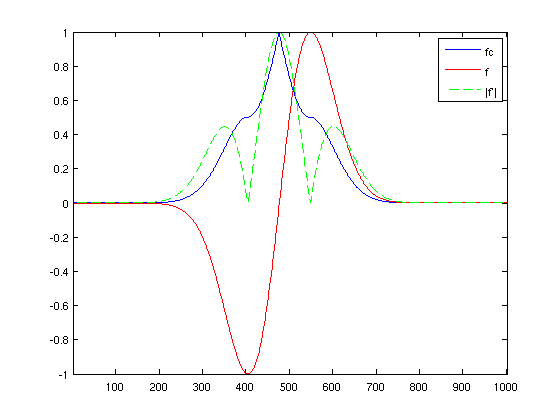
\includegraphics[scale=0.43]{./figures/SATAE/diff_cc.png}
\caption{Illustration of the complimentary function ($f_c$) as defined by
Equation 3 for a non-monotonic activation function ($f$). The absolute
derivative of $f$ is shown for comparison.}  \label{fig:diff_cc} \end{figure} 

An example of a complimentary function defined using the above formulation is
shown in Figure~\ref{fig:diff_cc}. Whereas $|f'(x)|$ is minimized at the
extrema of $f$, the complimentary function only plateaus at these locations.

\subsection{Relationship with the Contractive Auto-Encoder} Let $h_i$ be the
output of the $i^{th}$ hidden unit of a single-layer auto-encoder with
point-wise nonlinearity $f(\cdot)$. The regularizer imposed by the contractive
auto-encoder (CAE) can be expressed as follows: 

\begin{equation} \nonumber \sum_{ij} \left(\frac{\partial h_i}{\partial x_j}
\right)^2 = \sum_i ^{d_h} \left(f'(\sum_{j=1}^d W^e_{ij}x_j + b_i)^2 \| W^e_i
\| ^2 \right), \end{equation}  
 
\noindent where $x$ is a $d$-dimensional data vector, $f'(\cdot)$ is the
derivative of $f(\cdot)$, $b_i$ is the bias of the $i^{th}$ encoding unit, and
$W^e_i$ denotes the $i^{th}$ row of the encoding weight matrix. The first term
in the above equation tries to adjust the weights so as to push the activations
into the low gradient (saturation) regime of the nonlinearity, but is only
defined for differentiable activation functions. Therefore the CAE indirectly
encourages operation in the saturation regime. Computing the Jacobian, however,
can be cumbersome for deep networks. Furthermore, the complexity of computing
the Jacobian is $O(d \times d_h)$, although a more efficient implementation is
possible \cite{CAE}, compared to the $O(d_h)$ for the saturation penalty.  
 
\subsection{Relationship with the Sparse Auto-Encoder} In Section 3.2 it was
shown that SATAEs with shrink or rectified-linear activation functions are
equivalent to a sparse auto-encoder. Interestingly, the fact that the
saturation penalty happens to correspond to $L_1$ regularization in the case of
SATAE-shrink agrees with the findings in \cite{LISTA}. In their efforts to find
an architecture to approximate inference in sparse coding, Gregor et al. found
that the shrink function is particularly compatible with $L_1$ minimization.
Equivalence to sparsity only for some activation functions suggests that SATAEs
are a generalization of sparse auto-encoders. Like the sparsity penalty, the
saturation penalty can be applied at any point in a deep network for the same
computational cost. However, unlike the sparsity penalty the saturation penalty
is adapted to the nonlinearity of the particular layer to which it is applied. 

\chapter{Convolutional Sparse Inference}
\label{chapter:LISTA} 
Sparse coding inspired many early works in deep feature learning
\cite{SC,SAE,SAE2}, as well as early works in unsupervised learning of
convolutional feature hierarchies \cite{ConvSC}. All of these works rely
heavily on solving the sparse inference problem described in Chapter
\ref{chapter:related_work}.  However traditional iterative solvers can be
computationally expensive and are not formulated as functional mappings that
are amenable to network implementations \cite{FISTA}. The work by Gregor and
LeCun dubbed ``LISTA'' \cite{LISTA} proposed a specialized network architecture
for learning to predict sparse codes. However that work LISTA networks were
trained to directly predict the codes found using intirative inference
algorithms.  In this chapter we will empirically evaluate LISTA encoders under
a wider variety of conditions. This will include training convolutional LISTA
networks to learn sparse inference in convolutional dictionaries by directly
minimizing the lasso loss.

\section{Convolutional-LISTA} 

\begin{figure}
\centering
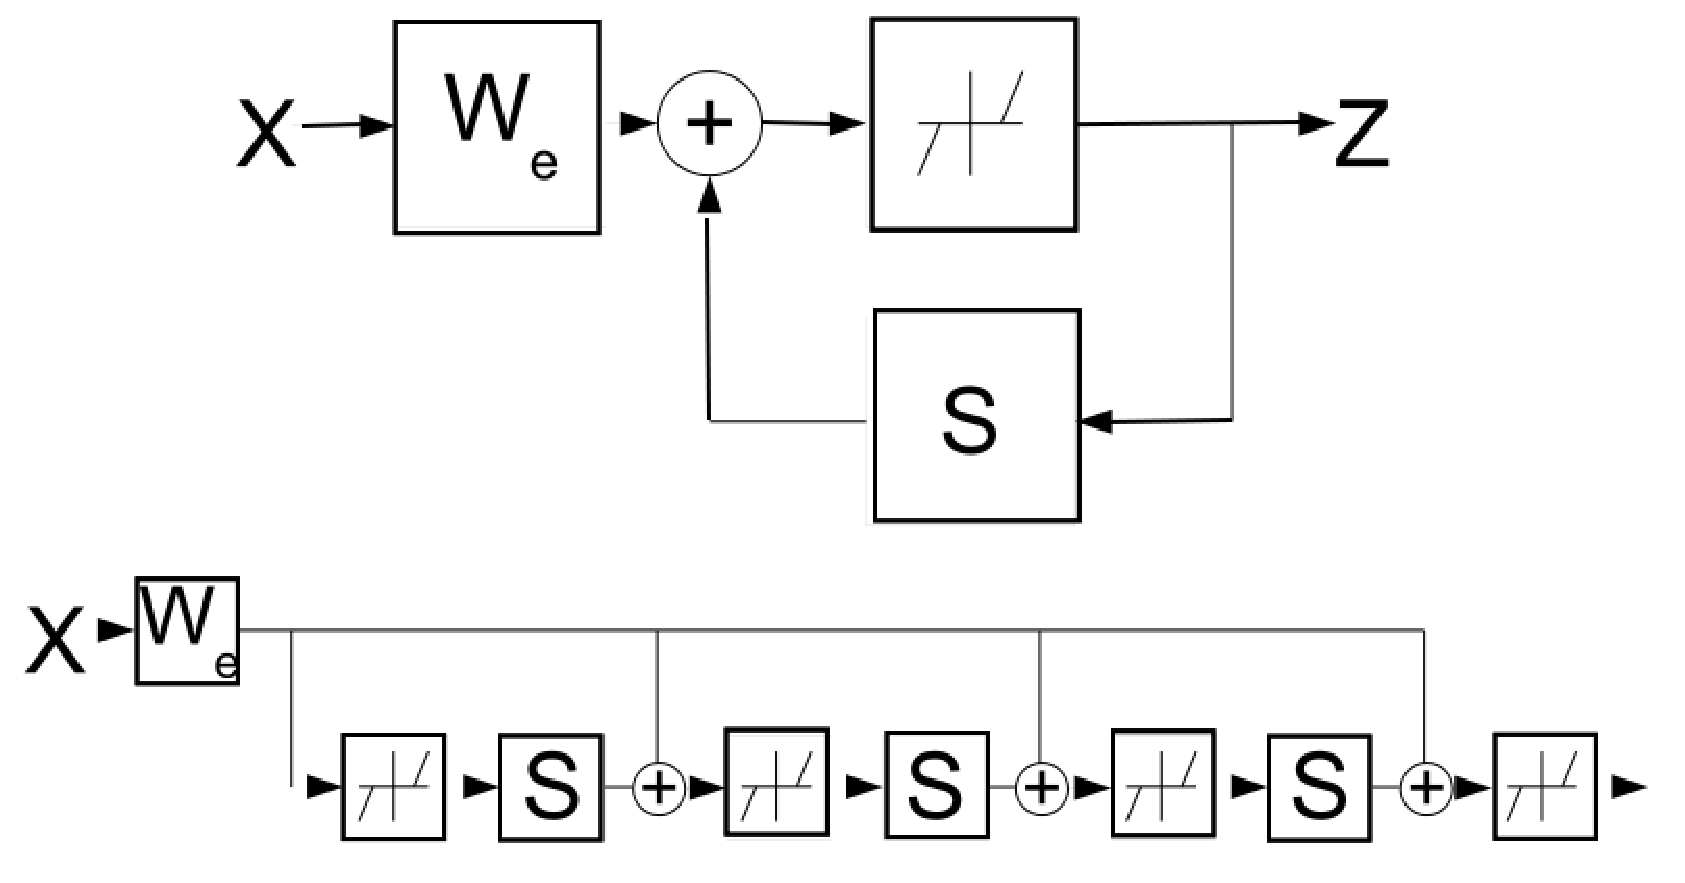
\includegraphics[scale=0.3]{./figures/LISTA/LISTA.pdf}
\caption{LISTA network architecture} 
\label{fig:LISTA} 
\end{figure}  

Recall the iterative ISTA algorithm for solving the relaxed sparse inference problem
known as the lasso was discussed in Chapter \ref{chapter:introduction}. 
The lasso loss is given by:
  
\begin{equation}
L_{lasso} = \frac{1}{2}\|X-W_dZ\| + \alpha |Z|_1 
\label{eqn:lasso} 
\end{equation} 

The LISTA network architecture is \emph{derived} by expressing the ISTA
algorithm as a recurrent network, and ``unrolling'' into a finite number of
loops with shared-weight stages.  The recurrent and unrolled networks
(three-loops) are shown in Figure \ref{fig:LISTA}. Note that
$S=I-\frac{1}{L}W_d^T W_d$, where $W_d$ is the decoder and $L$ is the upper
bound of $W_d^t W_d$. The above network can be made convolutional by replacing
the linear operators $W_e$ and $S$ with convolutional filter banks. In order to
be able to compute the reconstruction error in Equation \ref{eqn:lasso}, the
convolutional synthesis operator must produce outputs of the same size as the
input. This can be accomplished by using ``same'' convolutions or by cropping
the input and computing the reconstruction error in the ``valid'' regions. As
in ordinary convolutional networks, each convolutional layer produces multiple
output planes. For example, if the encoder takes in images of 3-input planes
and produces $n$-output planes then the $S$ convolution stage takes in
$n$-input planes and produces $n$-output planes. Convolutional dictionaries are
massively overcomplete, making sparse inference a potentially much
harder problem \cite{ConvSC}. 

\section{Learning to Perform Sparse Inference} Training networks to perform
sparse inference was originally proposed in \cite{groupSparsity}, the
specialized LISTA architecture was proposed later in \cite{LISTA}. In \cite{LISTA} 
networks were trained to explicitly minimize the $L^2$ distance between
the predicted and ground truth codes obtained via iterative sparse inference. 
This requires pre-training a dictionary and constructing a dataset consisting of 
sparse codes corresponding to minima of the lasso loss. 
However, in \cite{groupSparsity} the networks were implicitly trained to produce sparse
codes by directly minimizing a variant of the lasso loss. The variant included an additional 
term which encouraged the predicted codes to be close to the codes which minimize the lasso loss. 
In the context of dictionary learning it is desirable to learn the encoder and decoder jointly, 
(i.e. training an auto-encoder) as opposed to learning a decoder first then training an encoder to predict
the sparse codes. This section will present experimental results which empirically answer the following questions: 
\begin{itemize} 
\item{Does the convolutional LISTA architecture outperform other architectures when minimizing the lasso loss with a fixed dictionary?} 
\item{Does the convolutional LISTA architecture outperform other architectures when minimizing the lasso loss with a learned dictionary?} 
\end{itemize}
The following experiments were performed on the whitened CIFAR-10 dataset. 
A pre-trained decoder was obtained via convolutional sparse coding with FISTA inference \cite{ConvSC}.
This decoder was used to perform the fixed-dictionary experiments. The decoder consists of 32-convolutional $3\times9\times9$ filters shown in Figure \ref{fig:FISTA_decoder}.  
The top plot of Figure \ref{fig:learning_curves} presents the learning curves  

\begin{figure}
\centering
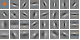
\includegraphics[scale=2]{./figures/LISTA/FISTA_decoder.png}
\caption{Pre-trained decoder used for fixed-decoder experiments} 
\label{fig:FISTA_decoder} 
\end{figure}  

\begin{figure}
\centering
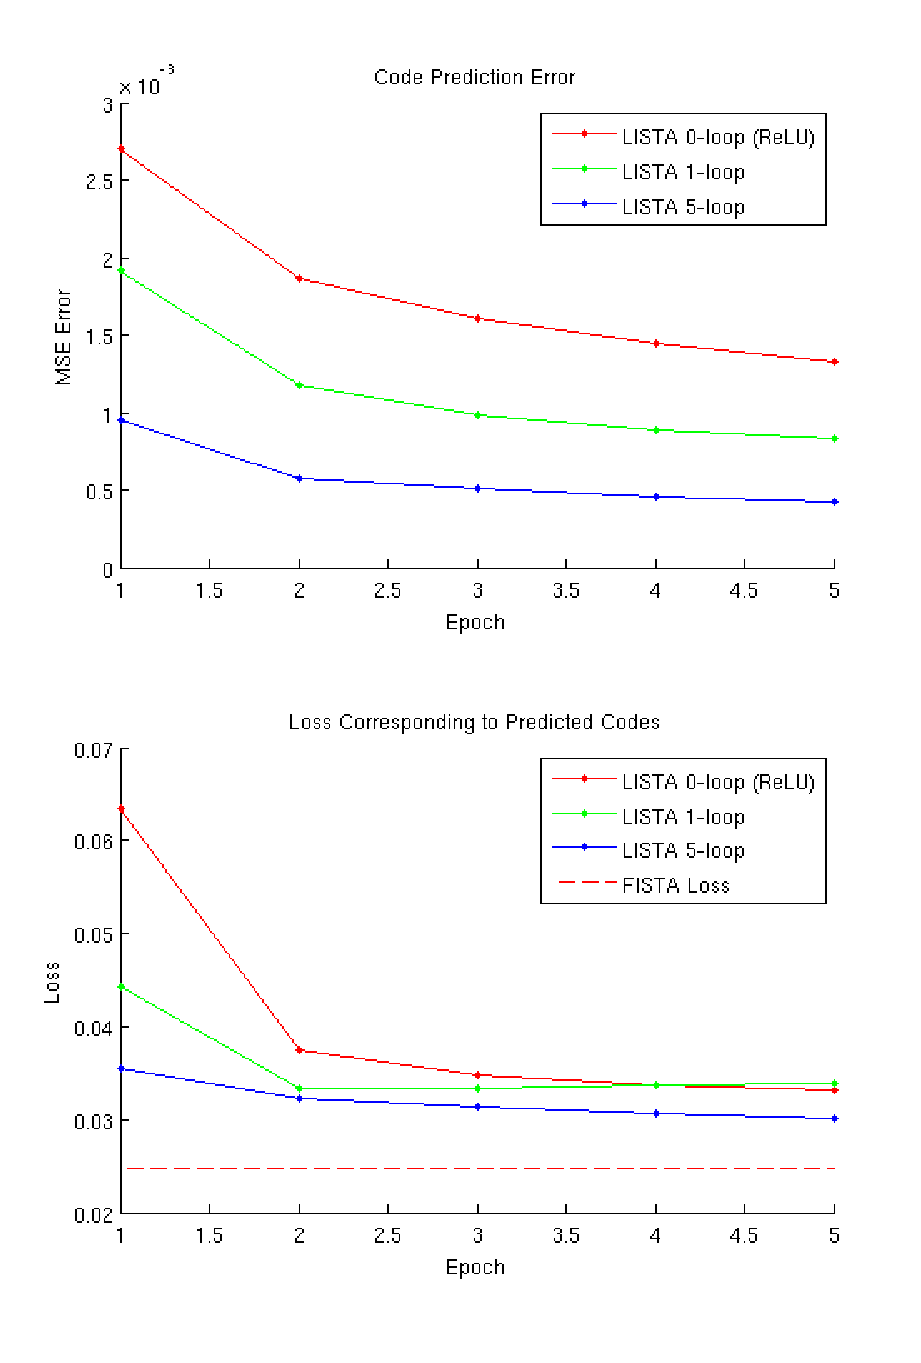
\includegraphics[scale=0.75]{./figures/LISTA/code_pred.pdf}
\caption{Sparse inference learning curves} 
\label{fig:learning_curves} 
\end{figure}  

\begin{figure}
\centering
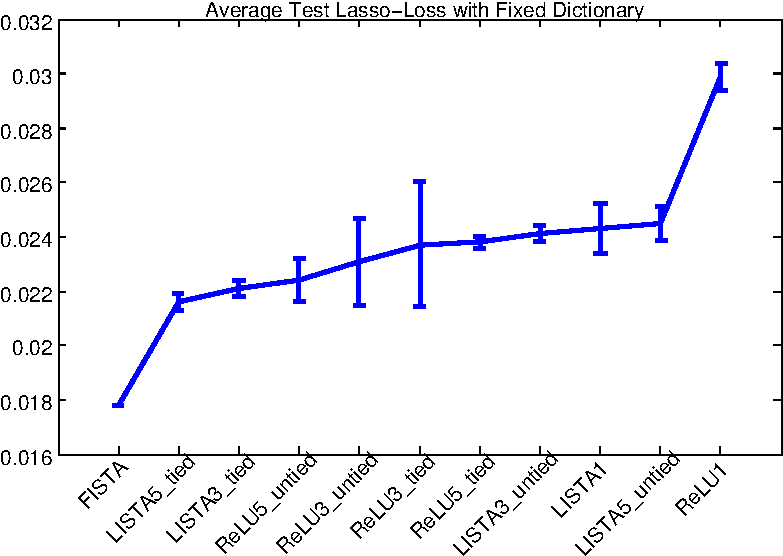
\includegraphics[scale=0.75]{./figures/LISTA/fixed_decoder_loss.pdf}
\caption{Lasso Loss} 
\label{fig:lasso_loss} 
\end{figure}  

\begin{figure}
\centering
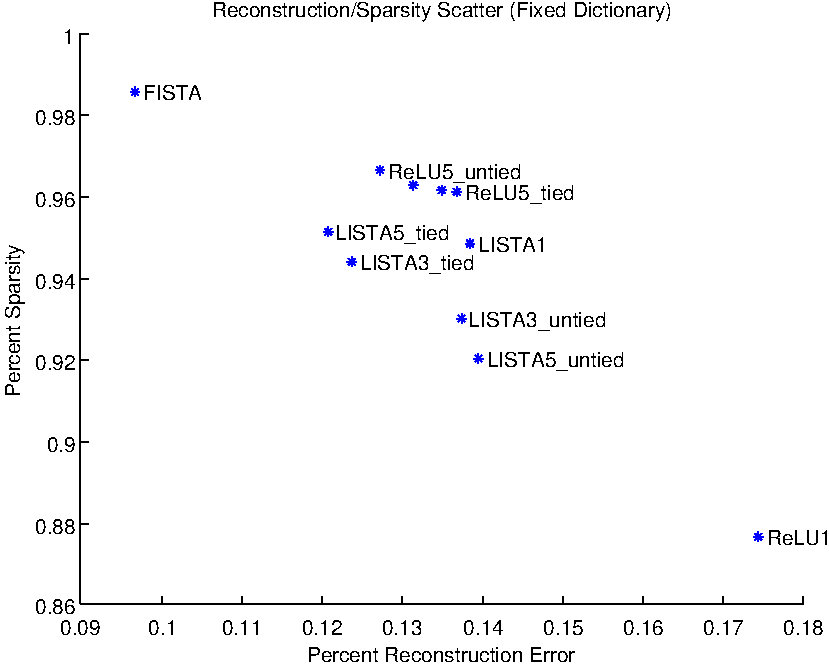
\includegraphics[scale=0.75]{./figures/LISTA/fixed_decoder_scatter.pdf}
\caption{Scatter Plot} 
\label{fig:scatter_fixed} 
\end{figure}  

 
\chapter{Learning Spatiotemporally Coherent Metrics}
\label{chapter:slow} 
\section{Introduction} Is it possible to characterize ``good'' representations
without specifying a task a priori? If so, does there exist a set of generic
priors which lead to these representations? In recent years state-of-the-art
results from supervised learning suggest that the most powerful representations
for solving specific tasks can be learned from the data itself. It has been
hypothesized that large collections of unprocessed and unlabeled data can be
used to learn generically useful representations. However the principles which
would lead to these representations in the realm of unsupervised learning
remain elusive. Temporal coherence is a form of weak supervision, which we
exploit to learn generic signal representations that are stable with respect to
the variability in natural video, including local deformations. 

Our main assumption is that data samples that are temporal neighbors are also
likely to be neighbors in the latent space. For example, adjacent frames in a
video sequence are more likely to be semantically similar than non-adjacent
frames. This assumption naturally leads to the slowness prior on features which
was introduced in SFA (\cite{SFA}). 

This prior has been successfully applied to metric learning, as a regularizer
in supervised learning, and in unsupervised learning
(\cite{DrLIM,DrLIMVideo,SFA}). A popular assumption in unsupervised learning is
that high dimensional data lies on a low dimensional manifold  parametrized by
the latent variables as in \cite{Bengio2012,CAE,DAE,SATAE}. In this case,
temporal sequences can be thought of as one-dimensional trajectories on this
manifold. Thus, an ensemble of sequences that pass through a common data sample
have the potential to reveal the local latent variable structure within a
neighborhood of that sample. 

Non-linear operators consisting of a redundant linear transformation followed
by a point-wise nonlinearity and a local pooling, are fundamental building
blocks in deep convolutional networks. This is due to their capacity to
generate local invariance while preserving discriminative information
(\cite{LeCun1998, JoanScat}). We justify that pooling operators are a natural
choice for our unsupervised learning architecture since they induce invariance
to local deformations. The resulting pooling auto-encoder model captures the
main source of variability in natural video sequences, which can be further
exploited by enforcing a convolutional structure. Experiments on YouTube data
show that one can learn pooling representations with good discrimination and
stability to observed temporal variability. We show that these features
represent a metric which we evaluate on retrieval and classification tasks. 

\section{Contributions and Prior Work} The problem of learning temporally
stable representations has been extensively studied in the literature, most
prominently in Slow Feature Analysis (SFA) and Slow Subspace Analysis (SSA)
(\cite{SFA,SSA,hyvarinen2003bubbles}). Works that learn slow features
distinguish themselves mainly in three ways: (1) how the features are
parametrized, (2) how the trivial (constant) solution is avoided, and (3)
whether or not additional priors such as independence or sparsity are imposed
on the learned features. 

The features presented in SFA take the form of a nonlinear transformation of
the input, specifically a quadratic expansion followed by a linear combination
using learned weights optimized for slowness (\cite{SFA}).  This
parametrization is equivalent to projecting onto a learned basis followed by
$L_2$ pooling. The recent work by \cite{complexCells} uses features which are
composed of projection onto a learned unitary basis followed by a local $L_2$
pooling in groups of two. 

Slow feature learning methods also differ in the way that they avoid the
trivial solution of learning to extract constant features. Constant features
are perfectly slow (invariant), however they are not informative
(discriminative) with respect to the input. All slow feature learning methods
must make a trade-off between the discriminability and stability of the learned
features in order to avoid trivial solutions. Slow Feature Analysis introduces
two additional constraints, namely that the learned features must have unit
variance and must be decorrelated from one another. In the work by
\cite{complexCells}, the linear part of the transformation into feature space
is constrained to be unitary. Enforcing that the transform be unitary implies
that it is invertible \emph{for all inputs}, and not just the data samples.
This unnecessarily limits the invariance properties of the transform and
precludes the possibility of learning over-complete bases. Since the pooling
operation following this linear transform has no trainable parameters,
including this constraint is sufficient to avoid the trivial solution. Metric
learning approaches (\cite{DrLIM}) can be used to perform dimensionality
reduction by optimizing a criteria which minimizes the distance between
temporally adjacent samples in the transformed space, while repelling
non-adjacent samples with a hinge loss, as explained in Section
\ref{sec:slowmetric}. The margin based contrastive term in DrLIM is explicitly
designed to only avoid the constant solution and provides no guarantee on how
informative the learned features are. Furthermore since distances grow
exponentially due to the curse of dimensionality, metric based contrastive
terms can be trivially satisfied in high dimensions.

Our approach uses a reconstruction criterion as a contrastive term. This
approach is most similar to the one taken by \cite{groupSparsity} when
optimizing group sparsity. In this work group-sparsity is replaced by slowness,
and multiple layers of convolutional slow features are trained. 

Several other studies combine the slowness prior with independence inducing
priors \cite{complexCells, Cadieu, zou2012deep}. For a detailed discussion on
the connection between independence and sparsity see \cite{Huyvarinen}.
However, our model maximizes the sparsity of the representation \emph{before}
the pooling operator. Our model can be interpreted as a sparse auto-encoder
additionally regularized by slowness through a local pooling operator.   

In this work we introduce the use of convolutional pooling architectures for
slow feature learning.  At small spatial scales, local translations comprise
the dominant source of variability in natural video; this is why many previous
works on slowness learn mainly locally translation-invariant features
(\cite{SFA,SSA,complexCells}). However, convolutional pooling architectures are
locally translation-invariant by design, which allows our model to learn
features that capture a richer class of invariances, beyond translation.
Finally, we demonstrate that nontrivial convolutional dictionaries can be
learned in the unsupervised setting using only stochastic gradient descent (on
mini-batches), despite their huge redundancy --- that is, without resorting to
alternating descent methods or iterative sparse inference algorithms. 


\section{Slowness as Metric Learning } \label{sec:slowmetric}

\begin{figure}
\centering
%\subfigure[ ]{
\begin{subfigure}[b]{0.49 \textwidth}
\centering
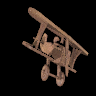
\includegraphics[scale=0.5]{./figures/slow/toyplane.png} 
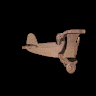
\includegraphics[scale=0.5]{./figures/slow/toyplane2.png} 
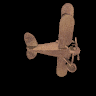
\includegraphics[scale=0.5]{./figures/slow/toyplane3.png}
        \caption{}
\label{fig:toyplane}
\end{subfigure}
%\caption{ }
%\end{figure} 
%
%\begin{figure}
%\centering 
%\begin{subfigure}[]
%\subfigure[ ]{
%\hspace{0.5cm}
\begin{subfigure}[b]{0.49 \textwidth}
\centering
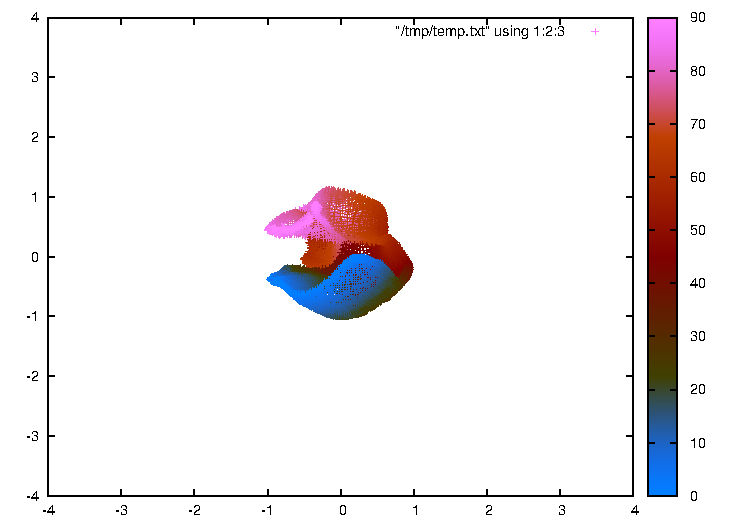
\includegraphics[scale=0.5,trim = 120 100 130 70, clip]{./figures/slow/drlim1.pdf}
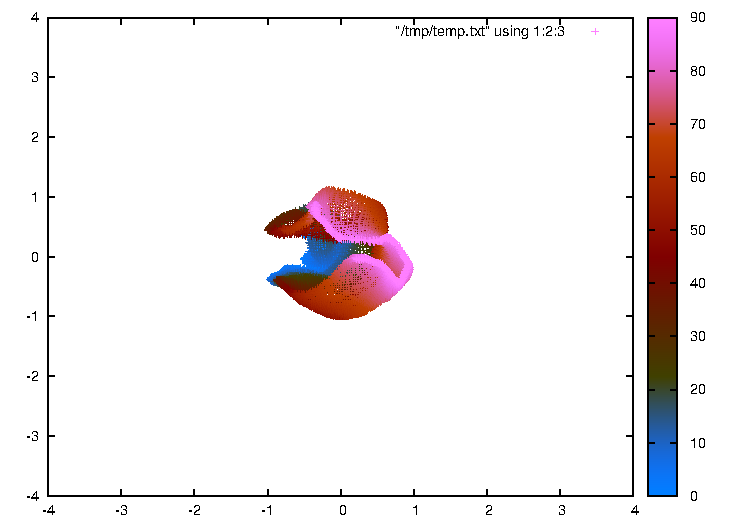
\includegraphics[scale=0.5,trim = 120 100 130 70, clip]{./figures/slow/drlim2.pdf}\\
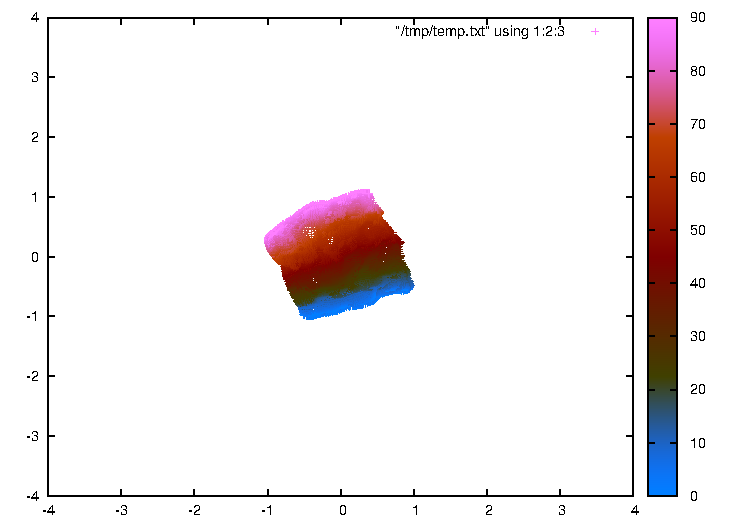
\includegraphics[scale=0.5,trim = 120 100 130 70, clip]{./figures/slow/drlim3.pdf} 
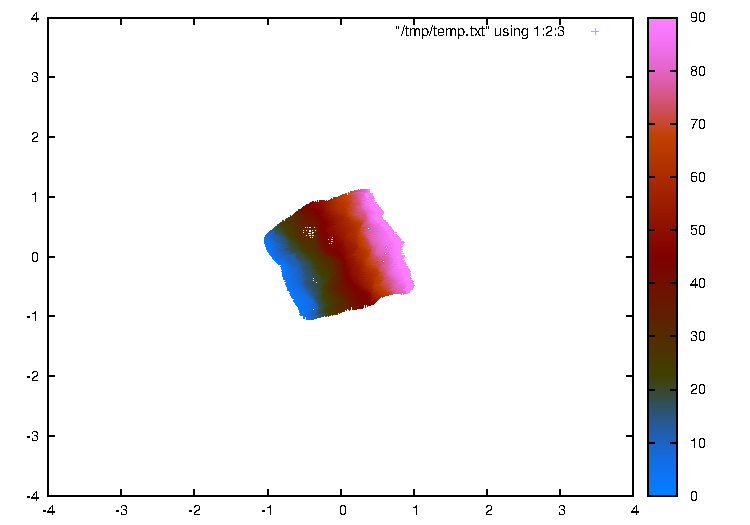
\includegraphics[scale=0.5,trim = 120 100 130 70, clip]{./figures/slow/drlim4.pdf}
        \caption{}
        \label{fig:drlim} 
\end{subfigure}

\caption{(a) Three samples from our rotating plane toy dataset. (b) Scatter plot of the dataset plotted in the output space of $G_W$ at the start (top) and end (bottom) of training. The left side of the figure is colored by the yaw angle, and the right side by roll, $0^{\circ}$  blue, $90^{\circ}$ in pink.}  
\end{figure} 

% Maybe reword so its not repetitive (first sent.) Temporal
coherence can be exploited by assuming a prior on the features extracted from
the temporal data sequence. One such prior is that the features should vary
slowly with respect to time. In the discrete time setting this prior
corresponds to minimizing an $L^p$ norm of the difference of feature vectors
for temporally adjacent inputs.  Consider a video sequence with $T$ frames, if
$z_t$ represents the feature vector extracted from the frame at time $t$ then
the slowness prior corresponds to minimizing $\sum_{t=1}^{T} \| z_t - z_{t-1}
\|_p$. To avoid the degenerate solution $z_t = z_0 ~\mbox{for}~ t=1...T$, a
second term is introduced which encourages data samples that are \emph{not}
temporal neighbors to be separated by at least a distance of $m$-units in
feature space, where $m$ is known as the margin. In the temporal setting this
corresponds to minimizing $max(0,m-\|z_t - z_{t'}\|_p)$, where $|t-t'| > 1$.
Together the two terms form the loss function introduced in \cite{DrLIM} as a
dimension reduction and data visualization algorithm known as DrLIM.  Assume
that there is a differentiable mapping from input space to feature space which
operates on \emph{individual} temporal samples. Denote this mapping by $G$ and
assume it is parametrized by a set of trainable coefficients denoted by $W$.
That is, $z_t = G_W(x_t)$. The per-sample loss function can be written as:
\begin{equation} \label{eqn:drlimcrit} L(x_t,x_{t'},W)=\left\{
\begin{array}{ll} \|G_W(x_t) - G_W(x_{t'})\|_p, &\text{if}~|t-t'| = 1  \\
\max(0,m-\|G_W(x_t) - G_W(x_{t'})\|_p) &\text{if}~|t-t'| > 1 \end{array}
\right.  \end{equation} In practice the above loss is minimized by constructing
a "Siamese" network (\cite{siamese}) with shared weights whose inputs are pairs
of samples along with their temporal indices. The loss is minimized with
respect to the trainable parameters with stochastic gradient descent via
back-propagation. To demonstrate the effect of minimizing Equation
\ref{eqn:drlimcrit} on temporally coherent data, consider a toy data-set
consisting of only one object. The data-set is generated by rotating a 3D model
of a toy plane (Figure \ref{fig:toyplane}) by $90^{\circ}$ in one-degree
increments around two-axes of rotation, generating a total of 8100 data
samples. Input images ($96 \times 96$) are projected into two-dimensional
output space by the mapping $G_W$. In this example the mapping $G_W(X):
\mathbb{R}^{9216} \to \mathbb{R}^2 $. We chose $G_W$ to be a fully connected
two layer neural network. In effect this data-set lies on an intrinsically
two-dimensional manifold parametrized by two rotation angles. Since the
sequence was generated by continuously rotating the object, temporal neighbors
correspond to images of the object in similar configurations.  Figure
\ref{fig:drlim} shows the data-set plotted in the output space of $G_W$ at the
start (top row) and end (bottom row) of training. The left and right hand sides
of Figure~\ref{fig:drlim} are colorized by the two rotational angles, which are
never explicitly presented to the network. This result implies that $G_W$ has
learned a mapping in which the latent variables (rotation angles) are
linearized. Furthermore, the gradients corresponding to the two rotation angles
are nearly orthogonal in the output space, which implies that the two features
extracted by $G_W$ are independent.  

\section{Slow Feature Pooling Auto-Encoders} \label{sfautoencs} The second
contrastive term in Equation \ref{eqn:drlimcrit} only acts to avoid the
degenerate solution in which $G_W$ is a constant mapping, it does not guarantee
that the resulting feature space is informative with respect to the input.
This discriminative criteria only depends on pairwise distances in the
representation space which is a geometrically weak notion in high dimensions.
We propose to replace this contrastive term with a term that penalizes the
reconstruction error of both data samples.  Introducing a reconstruction terms
not only prevents the constant solution but also acts to explicitly preserve
information about the input.  This is a useful property of features which are
obtained using unsupervised learning; since the task to which these features
will be applied is not known a priori, we would like to preserve as much
information about the input as possible. 

What is the optimal architecture of $G_{W}$ for extracting slow features? Slow
features are invariant to temporal changes by definition. In natural video and
on small spatial scales these changes mainly correspond to local translations
and deformations. Invariances to such changes can be achieved using appropriate
pooling operators \cite{JoanScat,LeCun1998}.  Such operators are at the heart
of deep convolutional networks (ConvNets), currently the most successful
supervised feature learning architectures \cite{ImageNet}. Inspired by these
observations, let $G_{W_e}$ be a two stage encoder comprised of a learned,
generally over-complete, linear map ($W_e$) and rectifying nonlinearity
$f(\cdot)$, followed by a local pooling. Let the $N$ hidden activations, $h =
f(W_ex)$, be subdivided into $K$ potentially overlapping neighborhoods denoted
by $P_i$. Note that biases are absorbed by expressing the input $x$ in
homogeneous coordinates. Feature $z_i$ produced by the encoder for the input at
time $t$ can be expressed as $G_{W_e}^i(t) = \|h_t\|^{P_i}_p =\left(\sum_{j \in
P_i} h_{tj}^{p} \right)^{\frac{1}{p}}$. Training through a local pooling
operator enforces a local topology on the hidden activations, inducing units
that are pooled together to learn complimentary features. In the following
experiments we will use $p=2$. Although it has recently been shown that it is
possible to recover the input when $W_e$ is sufficiently redundant,
reconstructing from these coefficients corresponds to solving a phase recovery
problem \cite{JoanPooling} which is not possible with a simple inverse mapping,
such as a linear map $W_d$. Instead of reconstructing from $z$ we reconstruct
from the hidden representation $h$. This is the same approach taken when
training group-sparse auto-encoders \cite{groupSparsity}. In order to promote
sparse activations in the case of over-complete bases we additionally add a
sparsifying $L_1$ penalty on the hidden activations. Including the rectifying
nonlinearity becomes critical for learning sparse inference in a hugely
redundant dictionary, e.g. convolutional dictionaries \cite{LISTA}. The
complete loss functional is: \begin{equation} \label{eqn:loss} L(x_t,x_{t'},W)=
\sum_{\tau = \{t,t'\}} \left(\|W_d h_\tau - x_\tau\|^2 + \alpha|h_\tau|
\right)+\beta \sum_{i=1}^K \left| \|h_t \|^{P_i} - \|h_{t'}\|^{P_i} \right|
\end{equation} Figure \ref{fig:diagram} shows a convolutional version of the
proposed architecture and loss.  This combination of loss and architecture can
be interpreted as follows: the sparsity penalty induces the first stage of the
encoder, $h=f(W_ex)$, to approximately infer sparse codes in the analysis
dictionary $W_e$; the slowness penalty induces the formation of pool groups
whose output is stable with respect to temporal deformations. In other words,
the first stage partitions the input space into disjoint linear subspaces and
the second stage recombines these partitions into temporally stable groups.
This can be seen as a sparse auto-encoder whose pooled codes are additionally
regularized by slowness.

\begin{figure} \centering \begin{subfigure}[b]{0.45\textwidth}
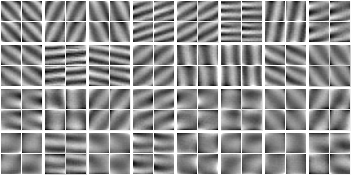
\includegraphics[width=\textwidth]{./figures/slow/slow_dec_pooling_sub.png}
\caption{} \label{fig:pooldec} \end{subfigure}
\begin{subfigure}[b]{0.45\textwidth}
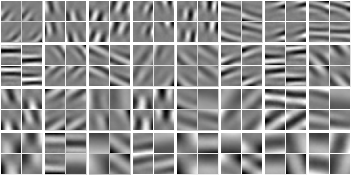
\includegraphics[width=\textwidth]{./figures/slow/slow_dec_l1_pooling.png}
\caption{} \label{fig:pooll1dec} \end{subfigure} \caption{Pooled decoder
dictionaries learned without (a) and with (b) the $L_1$ penalty using
(\ref{eqn:loss}).} \label{fig:sfpool} \end{figure}

\subsection{Fully-Connected Architecture}

To gain an intuition for the properties of the minima of Equation
\ref{eqn:loss} for natural data, an auto-encoder was trained on a small dataset
consisting of natural movie patches. This data set consists of approximately
170,000, $20 \times 20$ gray scale patches extracted from full resolution
movies.  Minimizing Equation \ref{eqn:loss} with $\alpha=0$ results in the
learned decoder basis shown in Figure \ref{fig:pooldec}. Here a dictionary of
512 basis elements was trained whose outputs were pooled in non-overlapping
groups of four resulting in 128 output features. Only the slowest 32 groups are
shown in Figure \ref{fig:pooldec}. The learned dictionary has a strong
resemblance to the two-dimensional Fourier basis, where most groups are
comprised of phase shifted versions of the same spatial frequency. Since
translations are an invariant of the local modulus of the Fourier transform,
the result of this experiment is indicative of the fact that translations are
the principal source of variation at small spatial scales. Minimizing Equation
\ref{eqn:loss} with $\alpha > 0$ results in a more localized basis depicted in
Figure \ref{fig:pooll1dec}. This basis is more consistent with a local
deformation model as opposed to a global one. 

\subsection{Convolutional Architecture} By replacing all linear operators in
our model with convolutional filter banks and including spatial pooling,
translation invariance need not be learned \cite{LeCun1998}. In all other
respects the convolutional model is conceptually identical to the fully
connected model described in the previous section. One important difference
between fully-connected and convolutional dictionaries is that the later can be
massively over-complete, making sparse inference potentially more challenging.
Nevertheless we found that non-trivial dictionaries (see Figure
\ref{fig:slowfilters}) can be learned using purely stochastic optimization,
that is, without a separate sparse inference phase. Let the linear stage of the
encoder consist of a filter bank which takes $C$ input feature maps
(corresponding to the 3 color channels for the first stage) and produces $D$
output feature maps. Correspondingly, the convolutional decoder transforms
these $D$ feature maps back to $C$ color channels. In the convolutional setting
slowness is measured by subtracting corresponding spatial locations in
temporally adjacent feature maps. In order to produce slow features a
convolutional network must compensate for the motion in the video sequence by
producing \emph{spatially} aligned activations for \emph{temporally} adjacent
samples. In other words, in order to produce slow features the network must
implicitly learn to track common patterns by learning features which are
invariant to the deformations exhibited by these patterns in the temporal
sequence. The primary mechanism for producing these invariances is pooling in
space and across features \cite{MaxOut}. Spatial pooling induces local
translation invariance. Pooling across feature maps allows the network to
potentially learn feature groups that are stable with respect to more general
deformations. Intuitively, maximizing slowness in a convolutional architecture
leads to \emph{spatiotemporally} coherent features.  
\begin{figure} \centering
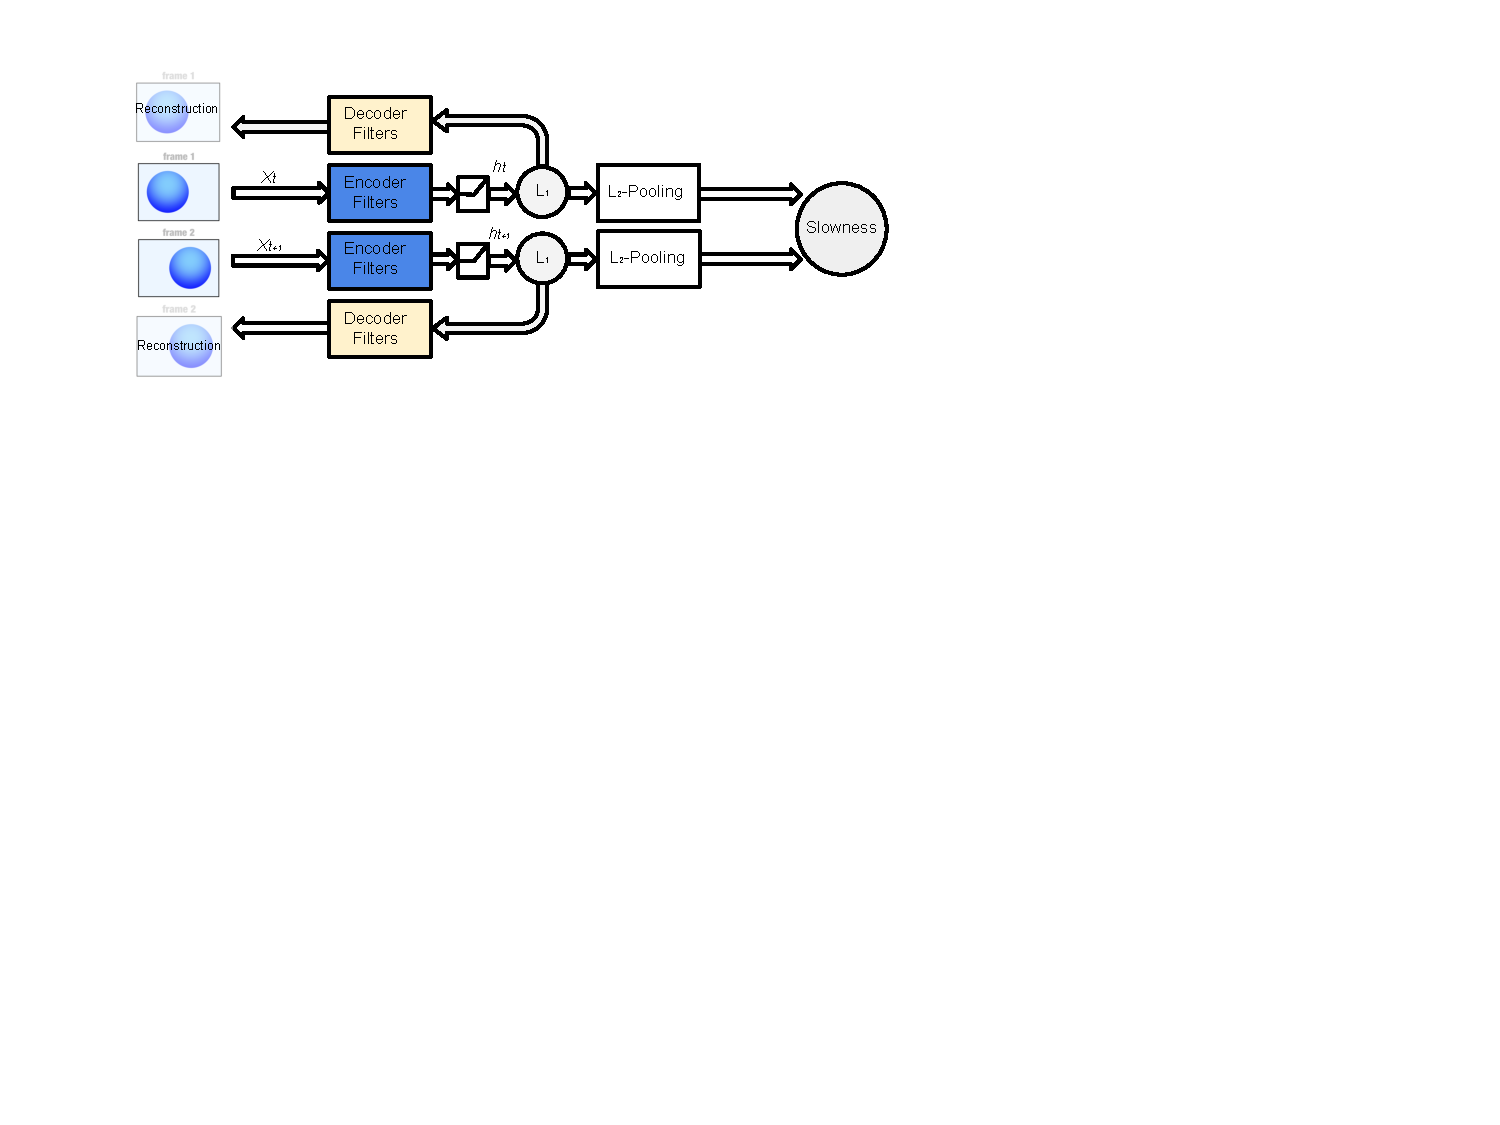
\includegraphics[scale=0.75,trim = 15 350 290 39,clip]{./figures/slow/Rebbutal_Figures/diagram.pdf} \caption{Block diagram of the Siamese convolutional model trained on pairs of frames. 
\label{fig:diagram}}
\end{figure} 
\section{Experimental Results} To verify the connection between
slowness and metric learning, we evaluate the metric properties of the learned
features. It is well known that distance in the extrinsic (input pixel) space
is not a reliable measure of semantic similarity. Maximizing slowness
corresponds to minimizing the distance between adjacent frames in code space,
therefore neighbors in code space should correspond to temporal neighbors. This
claim can be tested by computing the nearest neighbors to a query frame in code
space, and verifying whether they correspond to its temporal neighbors.
However, the features must also be discriminative so as not to collapse
temporally distant samples. In order to make this trade-off in a principled
manner, a dataset comprised of short natural scenes was collected.
Hyper-parameters are selected which maximize the so called "temporal coherence"
of the features which define the metric. We define the temporal coherence of a
metric $G_W(\cdot)$ as the area under the precision-recall curve, where
precision is defined as the proportion of the nearest neighbors that come from
the same scene, and recall is defined as the proportion of frames recalled from
that scene. In our experiments, we used the middle frame from each scene as the
query. 

However, temporal coherence can be a very weak measure of discriminability; it
merely requires that scenes be easy to disambiguate in feature space. If the
scenes are quite distinct, then maximizing temporal coherence directly can lead
to weakly discriminative features (e.g.~color histograms can exhibit good
temporal coherence). We therefore evaluate the learned features on a more
demanding task by assessing how well the metric learned from the YouTube
dataset transfers to a classification task on the CIFAR-10 dataset. Average
class-based precision is measured in feature space by using the test set as the
query images and finding nearest neighbors in the training set. Precision is
defined as the proportion of nearest neighbors that have the same label. As on
the YouTube dataset we evaluate the average precision for the nearest 40
neighbors. The CIFAR dataset contains considerably more interclass variability
than the scenes in our YouTube dataset, nevertheless many class instances are
visually similar.  

%\subsection{Description of Experiments} Our training dataset consists of
approximately $150,000$ frames extracted from YouTube videos. Of these,
approximately $20,000$ frames were held out for testing. The training and test
set frames were collected from separate videos. The videos were automatically
segmented into scenes of variable length (2-40 frames) by detecting large $L_2$
changes between adjacent frames. Each color frame was down-sampled to a $32
\times 32$ spatial resolution and the entire dataset was ZCA whitened
\cite{alexthesis}. Six scenes from the test set are shown in Figure
\ref{fig:youtube} where the first scene (top row) is incorrectly segmented.   

We compare the features learned by minimizing the loss in Equation
\ref{eqn:loss} with the features learned by minimizing DrLIM (Equation
\ref{eqn:drlimcrit}) and group sparsity (Equation \ref{eqn:groupL1}) losses.
Once trained, the convolution, rectification, and pooling stages are used to
transform the dataset into the feature space. We use cosine distance in feature
space to determine the nearest neighbors and select hyperparmeters for each
method which maximize the temporal coherence measure.

We trained two layers of our model using greedy layer-wise training
\cite{Bengio2012}. The first layer model contains a filter bank consisting of
64 kernels with $9 \times 9$ spatial support. The first $L_2$ pooling layer
computes the local modulus volumetrically, that is \emph{across} feature maps
in non-overlapping groups of four and spatially in $2 \times 2$ non-overlapping
neighborhoods. Thus the output feature vector of the first stage ($z_1$) has
dimensions $16 \times 16 \times 16$ (4096). Our second stage consists of 64 $5
\times 5$ convolutional filters, and performs $4 \times 4$ spatial pooling
producing a second layer code ($z_2$) of dimension $64 \times 4 \times 4$
(1024). The output of the second stage corresponds to a dimension reduction by
a factor of three relative to the input dimension.

Identical one and two-layer architectures were trained using the group sparsity
prior, similar to \cite{groupSparsity}. As in the slowness model, the two layer
architecture was trained greedily. Using the same notation as Equation
\ref{eqn:loss}, the corresponding loss can be written as:  \begin{equation}
L(x_t,W)= \sum_{\tau} \|W_d h_\tau - x_\tau\|^2 +\alpha \|h_\tau \|^{P_i}
\label{eqn:groupL1} \end{equation} Finally, identical one and two-layer
architectures were also trained by minimizing the DrLIM loss in Equation
\ref{eqn:drlimcrit}. Negative pairs, corresponding to temporally non-adjacent
frames, were independently selected at random. In order to achieve the best
temporal precision-recall performance, we found that each mini-batch should
consist of a large proportion of negative to positive samples (at least
five-to-one). Unlike the auto-encoder methods, the two layer architecture was
trained jointly rather than greedily.  \begin{figure} \centering
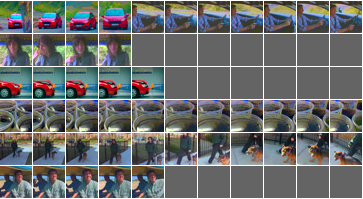
\includegraphics[scale=0.5]{./figures/slow/youtube.png} \caption{Six scenes from our
YouTube dataset \label{fig:youtube}}  \end{figure} \begin{figure}[ht]
\centering \newcommand{\figspace}{0.0cm} \newcommand{\figsize}{0.24\textwidth}
\begin{subfigure}[b]{\figsize}
\includegraphics[width=\textwidth]{./figures/slow/Rebbutal_Figures/filters_drlim.png}
\caption{} \label{fig:drlimfilters} \end{subfigure} \hspace{\figspace}
\begin{subfigure}[b]{\figsize}
\includegraphics[width=\textwidth]{./figures/slow/filters_not_slow.png} \caption{}
\label{fig:L1filters} \end{subfigure} \hspace{\figspace}
\begin{subfigure}[b]{\figsize}
\includegraphics[width=\textwidth]{./figures/slow/Rebbutal_Figures/filters_group_sparse.png}
\caption{} \label{fig:groupL1filters} \end{subfigure} \hspace{\figspace}
\begin{subfigure}[b]{\figsize}
\includegraphics[width=\textwidth]{./figures/slow/filters_slow.png} \caption{}
\label{fig:slowfilters} \end{subfigure} \caption{Pooled convolutional
dictionaries (decoders) learned with: (a) DrLIM and (b) sparsity only, (c)
group sparsity, and (d) sparsity and slowness. Groups of four features that
were pooled together are depicted as horizontally adjacent filters.}
\label{fig:filters} \end{figure}

\begin{figure} \center \begin{subfigure}[b]{0.45\textwidth}
\includegraphics[width=\textwidth, trim = 0 0 34 0,
clip]{./figures/slow/Rebbutal_Figures/NNtime1.pdf} \includegraphics[width=\textwidth, trim =
0 0 34 0, clip]{./figures/slow/Rebbutal_Figures/NNtime2.pdf} \caption{}
\label{fig:videoquery} \end{subfigure} \centering \hspace{0.1cm}
\begin{subfigure}[b]{0.45\textwidth} \includegraphics[width=\textwidth, trim =
0 0 34 0, clip]{./figures/slow/Rebbutal_Figures/NNclass1.pdf}
\includegraphics[width=\textwidth, trim = 0 0 34 0,
clip]{./figures/slow/Rebbutal_Figures/NNclass2.pdf} \caption{} \label{fig:cifarquery}
\end{subfigure} \caption{Query results in the (a) video and (b) CIFAR-10
datasets. Each row corresponds to a different feature space in which the
queries were performed; numbers (1 or 2) denote the number of
convolution-pooling layers. \label{fig:query}}  \label{fig:query} \end{figure}

\begin{figure} \centering \begin{subfigure}[b]{0.45\textwidth}
\includegraphics[width=\textwidth]{./figures/slow/Rebbutal_Figures/AUC_time-crop.pdf}
\caption{} \label{fig:ROCtime} \end{subfigure} \centering
\begin{subfigure}[b]{0.45\textwidth}
\includegraphics[width=\textwidth]{./figures/slow/Rebbutal_Figures/AUC_class-crop.pdf}
\caption{} \label{fig:ROCCIFAR} \end{subfigure} \caption{Precision-Recall
curves corresponding to the YouTube (a) and CIFAR-10 (b) dataset.}
\label{fig:ROC} \end{figure}

\begin{table} \centering \begin{tabular}{| l | l | l | l |} \hline Model &
Optimization & Temporal AUC & Class AUC \\ \hline Our Model Layer1 & --- &
0.262 & 0.296 \\ Our Model Layer2 & Greedy & 0.300 & \bf{0.310} \\ DrLIM Layer1
& --- & 0.188 & 0.221 \\ DrLIM Layer2 & Joint & \bf{0.378} & 0.268 \\ Group
$L_1$ Layer1 & --- & 0.231 & 0.266 \\ Group $L_1$ Layer2 & Greedy & 0.285 &
0.281 \\ \hline \end{tabular} \caption{Comnparison of Temporal and Class AUCs} \end{table} %\subsection{Discussion of Results}
%filter discussion  Figure \ref{fig:videoquery} shows the top nine query
results on the YouTube dataset for a single frame (left column) in eight
spaces. The top row shows the nearest neighbors in pixel space. The second row
shows the nearest neighbors in pixel space after ZCA whitening. The next six
rows show the nearest neighbors in feature space for one and two layer feature
transformations learned with slowness, group sparsity, and DrLIM. The resulting
first-layer filters and precision-recall curves are shown in Figures
\ref{fig:filters} and \ref{fig:ROC}, respectively.   Figures
\ref{fig:L1filters} and \ref{fig:slowfilters} show the decoders of two
one-layer models trained with $\beta = 0,2$, respectively, and a constant value
of $\alpha$. The filter bank trained with $\beta = 0$ exhibits no coherence
within each pool group; the filters are not visually similar nor do they tend
to co-activate at spatially neighboring locations. Most groups in the filter
bank trained with slowness tend be visually similar, corresponding to similar
colors and/or geometric structures. The features learned by minimizing the
DrLIM loss (Equation \ref{eqn:drlimcrit}), which more directly optimizes
temporal coherence, have much more high frequency content than the filters
learned with any of the auto-encoder methods. Nevertheless, some filters within
the same pool group exhibit similar geometric and color structure
(Figure~\ref{fig:drlimfilters}). The features learned with a group-sparsity
regularizer leads to nearly identical features (and nearly identical
activations) within each pool group (Figure~\ref{fig:groupL1filters}). This is
not surprising because group sparsity promotes co-activation of the features
within each pool group, by definition. We have also tried including an
individual sparsity prior, as in Equation~\ref{eqn:loss}, in order to encourage
independence among the pooled features. However this has lead to significantly
worse temporal-coherence performance.  %AUC discussion 

Figure \ref{fig:cifarquery} shows the result of two queries in the CIFAR-10
dataset. The corresponding precision-recall curves are shown in Figure
\ref{fig:ROCCIFAR}. One-layer DrLIM (4096 dimensional) exhibit poor performance
in both the temporal and class-based recall tasks. In contrast, jointly trained
two-layer DrLIM features (1024 dimensional) exhibit excellent temporal
coherence, outperforming all other models by a large margin. Although better
than the  first layer, second layer features perform significantly worse on the
CIFAR task than even the first-layer features learned by our model.
Furthermore, the nearest neighbors in both the one and two-layer feature spaces
learned with DrLIM are often neither visually nor semantically similar (see
Figure \ref{fig:cifarquery}). The conclusion which can be drawn from this
result is that \textbf{\emph{directly maximizing temporal coherence alone is
not a sufficient condition for achieving a semantically (or even visually)
coherent features}}. However, combining it with reconstruction and sparsity, as
in our model, yields the most semantically discriminative features. Although
significantly better than the features learned with DrLIM, the features learned
with group sparsity exhibit slightly weaker temporal coherence and
significantly worse class-based recall. Note that since all the features within
a pool group are practically identical, the invariants captured by the pool
groups are limited to local translations due to the spatial pooling. As a final
comparison, we trained a four layer ConvNet with supervision on CIFAR-10, this
network achieved approximately 80\% classification accuracy on the test set.
The architecture of the first two stages of the ConvNet is identical to the
architecture of the first and second unsupervised stages. The precision curve
corresponding to the first layer of the ConvNet is shown in Figure
\ref{fig:ROCCIFAR}, which is matched by our-model's second layer at high
recall. 

\section{Conclusion} Video data provides a virtually infinite source of
information to learn meaningful and complex visual invariances. While temporal
slowness is an attractive prior for good visual features, in practice it
involves optimizing conflicting objectives that balance invariance and
discriminability. In other words, perfectly slow features cannot be
informative. An alternative is to replace the small temporal velocity prior
with small temporal acceleration, leading to a criteria that \emph{linearizes}
observed variability. The resulting representation offers potential advantages,
such as extraction of both locally invariant and locally covariant features.
Although pooling representations are widespread in visual and audio recognition
architectures, much is left to be understood. In particular, a major question
is how to learn a stacked pooling representation, such that its invariance
properties are boosted while controlling the amount of information lost at each
layer. This could be possible by replacing the linear decoder of the proposed
model with a non-linear decoder which can be used to reconstruct the input from
pooled representations. Slow feature learning is merely one way to learn from
temporally coherent data. In this work we have provided an auto-encoder
formulation of the problem and shown that the resulting features are more
stable to naturally occurring temporal variability, while maintaining
discriminative power.

\chapter{Learning to Linearize under Uncertainty}
\label{chapter:linear} 

\section{Introduction}
In this chapter we continue our exploration of using time as a weak form of
supervision by introducing a new architecture and loss for training deep
feature hierarchies that linearize the transformations observed in unlabeled
natural video sequences. This is done by training a generative model to predict
video frames. We also address the problem of inherent uncertainty in prediction
by introducing latent variables that are non-deterministic functions of the
input into the network architecture. 

% * <mathieu.mic@free.fr> 2015-06-03T21:02:26.438Z: % %  TODO I understand the
%point you're making, but we don't really address it. Actually our features are
%bad for classification. Is that ok?  %

Recently there has been a flurry of work on learning features from video using
varying degrees of supervision
\cite{supFromTracker}\cite{FBvideo}\cite{predAlexNet}. Temporal coherence in
video can be considered as a form of weak supervision that can be exploited for
feature learning. More precisely, if we assume that data occupies some low
dimensional ``manifold'' in a high dimensional space, then videos can be
considered as one-dimensional trajectories on this manifold parametrized by
time. Many unsupervised learning algorithms can be viewed as various
parameterizations (implicit or explicit) of the data manifold
\cite{Bengio2012}. For instance, sparse coding implicitly assumes a locally
linear model of the data manifold \cite{sparseCoding}. In this work, we assume
that deep convolutional networks are good parametric models for natural data.
Parameterizations of the data manifold can be learned by training these
networks to \emph{linearize} short temporal trajectories, thereby implicitly
learning a local parametrization.   

In this work we cast the linearization objective as a frame \emph{prediction} problem. As in many other unsupervised learning schemes, this necessitates a generative model. Several recent works have also trained deep networks for the task of frame prediction \cite{FBvideo}\cite{supFromTracker}\cite{predAlexNet}. However, unlike other works that focus on prediction as a final objective, in this work prediction is regarded as a proxy for learning representations. We introduce a loss and architecture that addresses two main problems in frame prediction: (1) minimizing $L^2$ error between the predicted and actual frame leads to unrealistically blurry predictions, which potentially compromises the learned representation, and (2) copying the most recent frame to the input seems to be a hard-to-escape trap of the objective function,  which results in the network learning little more than the identity function. We argue that the source of blur partially stems from the inherent unpredictability of natural data; in cases where multiple valid predictions are plausible, a deterministic network will learn to average between all the plausible predictions. To address the first problem we introduce a set of latent variables that are non-deterministic functions of the input, which are used to explain the unpredictable aspects of natural videos. The second problem is addressed by introducing an architecture that explicitly formulates the prediction in the linearized feature space. 

The paper is organized as follows. Section \ref{sec:prior work} reviews relevant prior work. Section \ref{sec:main} introduces the basic architecture used for learning linearized representations.  Subsection \ref{subsec:phase pooling} introduces ``phase-pooling''--an operator that facilitates linearization by inducing a topology on the feature space. Subsection \ref{subsec:uncertainty} introduces a latent variable formulation as a means of learning to linearize under uncertainty. Section \ref{sec:experiments} presents experimental results on relatively simple datasets to illustrate the main ideas of our work. Finally, Section \ref{sec:conclusion} offers directions for future research. 
      
\section{Prior Work}
\label{sec:prior work} 
This work was heavily inspired by the philosophy revived by Hinton et al. \cite{capsules}, which introduced ``capsule'' units. In that work, an equivariant
representation is learned by the capsules when the true latent states were provided to the network as implicit targets. Our work allows us to move to a more unsupervised setting in which the true latent states are not only unknown, but represent completely arbitrary qualities. This was made possible with two assumptions: (1) that temporally adjacent samples also correspond to neighbors in the latent space, (2) predictions of future samples can be formulated as \emph{linear} operations in the latent space. In theory, the representation learned by our method is very similar to the representation learned by the ``capsules''; this representation has a locally stable \emph{``what''} component and a locally linear, or equivariant
 \emph{``where''} component. Theoretical properties of linearizing features were studied in \cite{taco}.    

Several recent works propose schemes for learning representations from video which use varying degrees of supervision\cite{FBvideo}\cite{supFromTracker}\cite{predAlexNet}\cite{slowAE}. For instance, \cite{predAlexNet} assumes that the pre-trained network from \cite{ImageNet} is already available and training consists of learning to mimic this network. Similarly, \cite{supFromTracker} learns a representation by receiving supervision from a tracker. This work is more closely related to fully unsupervised approaches for learning representations from video such as \cite{slowAE}\cite{SSA}\cite{Cadieu}\cite{SFA}\cite{DrLIMVideo}. It is most related to \cite{FBvideo} which also trains a decoder to explicitly predict video frames. Our proposed architecture was inspired by those presented in in \cite{ranzato2007} and \cite{zeiler2010}. 

\section{Learning Linearized Representations} 
\label{sec:main}
Our goal is to obtain a representation of each input sequence that varies linearly in time by transforming each frame \emph{individually}. Furthermore, we assume that this transformation can be learned by a deep, feed forward network referred to as the \emph{encoder}, denoted by the function $F_W$.
Denote the code for frame $x^t$ by $z^t = F_W(x^t)$. Assume that the dataset is parameterized by a temporal index $t$ so it is described by the sequence $X = \{...,x^{t-1},x^t,x^{t+1},...\}$ with a corresponding feature sequence produced by the encoder $Z = \{...,z^{t-1},z^t,z^{t+1},...\}$. Thus our goal is to train $F_W$ to produce a sequence $Z$ whose average local curvature is smaller than sequence $X$. A scale invariant local measure of curvature is the cosine distance between the two vectors formed by three temporally adjacent samples. However, minimizing the curvature directly can result in the trivial solutions: $z_t=ct~\forall~t$ and $z_t=c~\forall~t$. These solutions are trivial because they are virtually \emph{uninformative} with respect to the input $x^t$ and therefore cannot be a \emph{meaningful representation of the input}. To avoid this solution, we also minimize the prediction error in the input space. The predicted frame is generated in two steps: (i) linearly extrapolation in code space to obtain a predicted code $\hat z^{t+1} = \mathbf a [z^t~~z^{t-1}]^T$ followed by (ii) a \emph{decoding} with $G_W$, which generates the predicted frame $\hat x^{t+1} = G_W(\hat z^{t+1})$. For example, if $\mathbf{a} = [2,-1]$ the predicted code $\hat z^{t+1}$ corresponds to a constant speed linear extrapolation of $z^t$ and $z^{t-1}$. The $L^2$ prediction error is minimized by jointly training the encoder and decoder networks. Note that minimizing prediction error alone will not necessarily lead to low curvature trajectories in $Z$ since the decoder is unconstrained; the decoder may learn a many to one mapping which maps different codes to the same output image without forcing them to be equal. To prevent this, we add an explicit curvature penalty to the loss, corresponding to the cosine distance between $(z^t-z^{t-1})$ and $(z^{t+1}-z^t)$.    
The complete loss to minimize is: 
\begin{equation}
L = \frac{1}{2}\| G_W(\mathbf a \begin{bmatrix}z^t&z^{t-1}\end{bmatrix}^T) - x^{t+1} \|^2_2 - \lambda \frac{(z^t - z^{t-1})^T(z^{t+1} - z^t)}{\|z^t-z^{t-1}\| \|z^{t+1} - z^t\|}
\label{eqn:loss} 
\end{equation} 

This feature learning scheme can be implemented using an autoencoder-like network with shared encoder weights. 
\begin{figure}
  \centering
  \begin{subfigure}[b]{0.15\textwidth}
        \includegraphics[width=\textwidth]{./figures/linear/fig1.pdf}
        \caption{}
        \label{fig:3pixels}
  \end{subfigure}
  \begin{subfigure}[b]{0.45\textwidth}
        \includegraphics[width=\textwidth]{./figures/linear/fig2.pdf} 
        \caption{}
        \label{fig:manifold}
  \end{subfigure}
  \caption{(a) A video generated by translating a Gaussian intensity bump over a three pixel array ($x$,$y$,$z$), (b) the corresponding manifold parametrized by time in three dimensional space}
  \label{fig:threepixel}
\end{figure}

\subsection{Phase Pooling} 
\label{subsec:phase pooling} 
Thus far we have assumed a generic architecture for $F_W$ and $G_W$. We now consider custom architectures and operators that are particularly suitable for the task of linearization. To motivate the definition of these operators, consider a video generated by translating a Gaussian ``intensity bump'' over a three pixel region at constant speed. The video corresponds to a one dimensional manifold in three dimensional space, i.e. a curve parameterized by time (see Figure \ref{fig:threepixel}). Next, assume that some convolutional feature detector fires only when centered on the bump.
Applying the $max$-pooling operator to the activations of the detector in this three-pixel region signifies the presence of the feature somewhere in this region (\emph{i.e. the ``what''}). Applying the $argmax$ operator over the region returns the position (\emph{i.e. the ``where''}) with respect to some local coordinate frame defined over the pooling region. This position variable varies linearly as the bump translates, and thus parameterizes the curve in Figure \ref{fig:manifold}. These two channels, namely the \emph{what} and the \emph{where}, can also be regarded as generalized magnitude $m$ and phase $\mathbf p$, corresponding to a factorized representation: the magnitude represents the active set of parameters, while the phase represents the set of local coordinates in this active set.
 We refer to the operator that outputs both the $max$ and $argmax$ channels as the ``phase-pooling'' operator.

\begin{figure}
  \centering
   \includegraphics[width=0.7\textwidth]{./figures/linear/network.pdf}
   \caption{The basic linear prediction architecture with shared weight encoders}
   \label{fig:arch1}
   %TODO: shouldn't we add curvature penalty?
\end{figure}

In this example, spatial pooling was used to linearize the translation of a fixed feature. More generally, the phase-pooling operator can locally linearize arbitrary transformations if pooling is performed not only spatially, but also across features in some topology.
%Moreover, we define an ``unpooling'' operation which reconstructs an approximate activation map from the $max$ and $argmax$ measurements, and therefore allows us to generate frame predictions from the parameter space. This is done by placing the values given by the $max$ at the locations given by the $argmax$.

In order to be able to back-propagate through $\mathbf{p}$, we define a soft version of the $max$ and $argmax$ operators within each pool group. For simplicity, assume that the encoder has a fully convolutional architecture which outputs a set of feature maps, possibly of a different resolution than the input. 
Although we can define an arbitrary topology in feature space, for now assume that we have the familiar three-dimensional spatial feature map representation where each activation is a function $z(f,x,y)$, where $x$ and $y$ correspond to the spatial location, and $f$ is the feature map index. Assuming that the feature activations are positive, we define our soft \emph{``max-pooling''} operator for the $k^{th}$ neighborhood $N_k$ as:
\begin{equation}
m_k = \sum_{N_k} z(f,x,y)\!~ \frac{e^{\beta z(f,x,y)}}{\sum_{N_k}e^{\beta z(f\prime, x\prime, y\prime )}}\,\approx\underset{N_k}\max~z(f,x,y),
\label{eqn:mag}
\end{equation}   
where $\beta \geq 0$.
Note that the fraction in the sum is a softmax operation (parametrized by $\beta$), which is positive and sums to one in each pooling region. The larger the $\beta$, the closer it is to a unimodal distribution and therefore the better $m_k$ approximates the \emph{max} operation. On the other hand, if $\beta=0$, Equation \ref{eqn:mag} reduces to \emph{average-pooling}. Finally, note that $m_k$ is simply the expected value of $z$ (restricted to $N_k$) under the softmax distribution.

Assuming that the activation pattern within each neighborhood is approximately unimodal, we can define a soft versions of the $argmax$ operator. The vector $\mathbf p_k$ approximates the local coordinates in the feature topology at which the max activation value occurred. Assuming that pooling is done volumetrically, that is, spatially \emph{and} across features, $\mathbf p_k$ will have three components. In general, the number of components in $\mathbf p_k$ is equal to the dimension of the topology of our feature space induced by the pooling neighborhood. The dimensionality of $\mathbf p_k$ can also be interpreted as the \emph{maximal intrinsic dimension of the data}. If we define a local standard coordinate system in each pooling volume to be bounded between -1 and +1, the soft ``\emph{argmax-pooling}'' operator is defined by the vector-valued sum:  
\begin{equation}
\mathbf p_k = \sum_{N_k}
\begin{bmatrix}
f \\ x \\ y
\end{bmatrix}
\frac{e^{\beta z(f,x,y)}}{\sum_{N_k}e^{\beta z(f\prime, x\prime, y\prime )}} \approx\underset{ N_k}\argmax~z(f,x,y),
\label{eqn:phase}
\end{equation}   
%TODO: Michael, can you find a better way to say that f,x,y are not only used to index z(f,x,y), but also take values from -1 to +1?  
where the indices $f,x,y$ take values from -1 to 1 in equal increments over the pooling region. 
Again, we observe that $\mathbf{p}_k$ is simply the expected value of $\begin{bmatrix}f&x&y\end{bmatrix}^T$ under the softmax distribution.

The phase-pooling operator acts on the output of the encoder, therefore it can simply be considered as the last encoding step. Correspondingly we define an ``\emph{un-pooling}'' operation as the first step of the decoder, which produces reconstructed activation maps by placing the magnitudes $m$ at appropriate locations given by the phases $\mathbf p$. 

Because the phase-pooling operator produces both magnitude and phase signals for each of the two input frames, it remains to define the predicted magnitude and phase of the third frame. In general, this linear extrapolation operator can be learned, however ``hard-coding'' this operator allows us to place implicit priors on the magnitude and phase channels. The predicted magnitude and phase are defined as follows: 
\begin{eqnarray}
m^{t+1}=&\frac{m^t + m^{t-1}}{2}&\\
\label{eqn:magpred} 
\mathbf p^{t+1}=&2\mathbf p^t-\mathbf p^{t-1}& 
\label{eqn:phasepred} 
\end{eqnarray} 
Predicting the magnitude as the mean of the past imposes an implicit stability prior on $m$, i.e. the temporal sequence corresponding to the $m$ channel should be stable between adjacent frames. The linear extrapolation of the phase variable imposes an implicit linear prior on $\mathbf p$. Thus such an architecture produces a factorized representation composed of a locally stable $m$ and locally linearly varying $\mathbf p$. When phase-pooling is used curvature regularization is only applied to the $\mathbf p$ variables. The full prediction architecture is shown in Figure \ref{fig:arch1}.  

%Thus if phase pooling is included in the encoder, and we assume that un-pooling is the first operator in the decoder, then Equation \ref{eqn:loss} can be rewritten as: 
%\begin{equation}
%L = \frac{1}{2}\| G_W \left(\begin{bmatrix} 0.5 & 0.5 \\ 2 & -1 \end{bmatrix} \begin{bmatrix} m^t & \mathbf{p^t}  \\ m^{t-1} & \mathbf{p^{t-1}} \end{bmatrix} \right)- x^{t+1} \|^2_2 - \lambda \frac{(\mathbf p^t - \mathbf p^{t-1})^T(\mathbf p^{t+1} - \mathbf p^t)}{\|\mathbf p^t- \mathbf p^{t-1}\| \|\mathbf p^{t+1} - \mathbf p^t\|}
%\label{eqn:loss} 
%\end{equation} 

\subsection{Addressing Uncertainty} 
%\begin{figure}
%  \centering
%   \includegraphics[width=0.4\textwidth]{./figures/linear/delta_ambiguity.pdf}
%   \caption{Cartoon of ambiguity in video}
%   \label{fig:delta}
%\end{figure} 
\label{subsec:uncertainty} 
Natural video can be inherently unpredictable; objects enter and leave the field of view, and out of plane rotations can also introduce previously invisible content. In this case, the prediction should correspond to the \emph{most likely outcome} that can be learned by training on similar video. However, if multiple outcomes are present in the training set then minimizing the $L^2$ distance to these multiple outcomes induces the network to predict the \emph{average outcome}. In practice, this phenomena results in blurry predictions and may lead the encoder to learn a less discriminative representation of the input. To address this inherent unpredictability we introduce latent variables $\delta$ to the prediction architecture that are not deterministic functions of the input. These variables can be adjusted \emph{using the target} $x^{t+1}$ in order to minimize the prediction $L^2$ error. The interpretation of these variables is that they explain all aspects of the prediction that are not captured by the encoder. For example, $\delta$ can be used to switch between multiple, equally likely predictions. It is important to control the capacity of $\delta$ to prevent it from explaining the entire prediction on its own. Therefore $\delta$ is restricted to act only as a correction term in the code space output by the encoder. To further restrict the capacity of $\delta$ we enforce that $dim(\delta) \ll dim(z)$. 
More specifically, the $\delta$-corrected code is defined as:
\begin{equation} 
\label{eqn:delta}
\hat z^{t+1}_\delta =  z^{t} + (W_1 \delta) \odot \mathbf{a}\begin{bmatrix}z^t&z^{t-1}\end{bmatrix}^T
\end{equation}  
Where $W_1$ is a trainable matrix of size $dim(\delta) \times dim(z)$, and $\odot$ denotes the component-wise product.  
During training, $\delta$ is inferred (using gradient descent) for each training sample by minimizing the loss in Equation \ref{eqn:delta_loss}. The corresponding adjusted $\hat z_\delta ^{t+1}$ is then used for back-propagation through $W$ and $W_1$. At test time $\delta$ can be selected via sampling, assuming its distribution on the training set has been previously estimated.
\begin{equation} 
\label{eqn:delta_loss}
L = \min\limits_\delta \| G_W(\hat z_\delta ^{t+1}) - x^{t+1} \|^2_2 - \lambda \frac{(z^t - z^{t-1})^T(z^{t+1} - z^t)}{\|z^t-z^{t-1}\| \|z^{t+1} - z^t\|} \\
\end{equation} 
The following algorithm details how the above loss is minimized using stochastic gradient descent:

\begin{algorithm}
\caption{Minibatch stochastic gradient descent training for prediction with uncertainty. The number of $\delta$-gradient descent steps ($k$) is treated as a hyper-parameter. }
\begin{algorithmic}
\FOR{number of training epochs}  
\STATE{Sample a mini-batch of temporal triplets $\{x^{t-1},x^t,x^{t+1}\}$}
\STATE{Set $\delta_0=0$}
\STATE{Forward propagate $x^{t-1},x^t$ through the network and obtain the codes $z^{t-1}, z^t$ and the prediction $\hat x_0^{t+1}$}
\FOR{$i$ =1 to $k$}
\STATE{Compute the $L^2$ prediction error}
\STATE{Back propagate the error through the decoder to compute the gradient $\frac{\partial L}{\partial \delta^{i-1}}$} 
\STATE{Update $\delta_i = \delta_{i-1} - \alpha \frac{\partial L}{\partial \delta^{i-1}}$}
\STATE{Compute $\hat z^{t+1}_{\delta_i} =  z^{t} + (W_1 \delta_i) \odot \mathbf{a}\begin{bmatrix}z^t&z^{t-1}\end{bmatrix}^T$}
\STATE{Compute $\hat x_i^{t+1} = G_W(z^{t+1}_{\delta^i})$}
\ENDFOR
\STATE{Back propagate the full encoder/predictor loss from Equation~\ref{eqn:delta_loss} using $\delta_k$, and update the weight matrices $W$ and $W_1$}
\ENDFOR
\end{algorithmic} 
\end{algorithm}
When phase pooling is used we allow $\delta$ to only affect the phase variables in Equation \ref{eqn:phasepred}, this further encourages the magnitude to be stable and places all the uncertainty in the phase.   

\section{Experiments} 
\label{sec:experiments}
The following experiments evaluate the proposed feature learning architecture and loss. In the first set of experiments we train a shallow architecture on natural data and visualize the learned features in order gain a basic intuition. In the second set of experiments we train a deep architecture on simulated movies generated from the NORB dataset. By generating frames from interpolated and extrapolated points in code space we show that a linearized representation of the input is learned. Finally, we explore the role of uncertainty by training on only partially predictable sequences, we show that our latent variable formulation can account for this uncertainty enabling the encoder to learn a linearized representation even in this setting.   

\subsection{Shallow Architecture Trained on Natural Data}
To gain an intuition for the features learned by a phase-pooling architecture let us consider an encoder architecture comprised of the following stages: convolutional filter bank,   rectifying point-wise nonlinearity, and phase-pooling. The decoder architecture is comprised of an un-pooling stage followed by a convolutional filter bank. This architecture was trained on simulated $32 \times 32$ movie frames taken from YouTube videos \cite{slowAE}. Each frame triplet is generated by transforming still frames with a sequence of three rigid transformations (translation, scale, rotation). More specifically let $A$ be a random rigid transformation parameterized by $\tau$, and let $x$ denote a still image reshaped into a column vector, the generated triplet of frames is given by $\{f_1=A_{\tau=\frac{1}{3}}x,f_2=A_{\tau=\frac{2}{3}}x,f_3=A_{\tau=1}x\}$. Two variants of this architecture were trained, their full architecture is summarized in the first two lines of Table \ref{tbl:arch}. In Shallow Architecture 1, phase pooling is performed spatially in non-overlapping groups of $4\times4$ and across features in a one-dimensional topology consisting of non-overlapping groups of four. Each of the 16 pool-groups produce a code consisting of a scalar $m$ and a three-component $\mathbf p = [p_f,p_x,p_y]^T$ (corresponding to two spatial and one feature dimensions); thus the encoder architecture produces a code of size $16 \times 4 \times 8 \times 8$ for each frame. The corresponding filters whose activations were pooled together are laid out horizontally in groups of four in Figure \ref{fig:filters}(a). Note that each group learns to exhibit a strong ordering corresponding to the linearized variable $p_f$. Because global rigid transformations can be locally well approximated by translations, the features learn to parameterize local translations. In effect the network learns to linearize the input by tracking common features in the video sequence. Unlike the spatial phase variables, $p_f$ can linearize sub-pixel translations. Next, the architecture described in column 2 of Table \ref{tbl:arch} was trained on natural movie patches with the natural motion present in the real videos. The architecture differs in only in that pooling across features is done with overlap (groups of 4, stride of 2). The resulting decoder filters are displayed in Figure \ref{fig:filters} (b). Note that pooling with overlap introduces smoother transitions between the pool groups. Although some groups still capture translations, more complex transformations are learned from natural movies. 

%\begin{table} 
%\tiny
%\centering
%\resizebox{\linewidth}{!}{
%\begin{tabular}{| l | c | c | c | c | c | c | }
%  \hline                       
%   & Shallow Architecture 1 & Shallow Architecture 2 & Deep Architecture 1 & Deep Architecture 2 & Deep Architecture 3 \\
%  \hline
%  Encoder & Conv+ReLU $64 \times 9 \times 9$ & Conv+ReLU $64 \times 9 \times 9$ & Conv+ReLU $16\times 9 \times 9$ & Conv+ReLU $16\times 9 \times 9$ & Conv+ReLU $16\times 9 \times 9$ \\
%  		  & Phase Pool $4$ & Phase Pool $4$ stride 2  & Conv+ReLU $32\times 9 \times 9$ & Conv+ReLU $32\times 9 \times 9$& Conv+ReLU $32\times 9 \times 9$  \\
%  		  &	& & F.C.+ReLU $8192 \times 4096$ & F.C.+ReLU $8192 \times 4096$ & F.C.+ReLU $8192 \times 4096$ \\
%  		  &	& & & & Reshape   $64 \times 8 \times 8$ \\
%  		  &	& & & & Phase Pool $8 \times 8$ \\ 
%		  \hline
%Prediction & Average Mag. & Average Mag. & None & Linear Extrapolation & Average Mag. \\
% & Linear Extrap. Phase & Linear Extrap. Phase& & & Linear Extrap. Phase\\
%  		  \hline
%  Decoder & Conv $64 \times 9 \times 9$  & Conv $64 \times 9 \times 9$ & F.C.+ReLU $\mathbf{8192} \times 8192$ & F.C.+ReLU $4096 \times 8192$ &Unpool $8 \times 8$ \\
%          & & &Reshape $32 \times 16 \times 16$  &Reshape $32 \times 16 \times 16$ &F.C.+ReLU $4096 \times 8192$ \\ 
%          & & &Spatial Padding $8 \times 8$  & Spatial Padding $8 \times 8$&Reshape $32 \times 16 \times 16$ \\
%          & & &Conv+ReLU $16 \times 9 \times 9$  &Conv+ReLU $16 \times 9 \times 9$ &Spatial Padding $8 \times 8$ \\
%          & & &Spatial Padding $8 \times 8$  &Spatial Padding $8 \times 8$ &Conv+ReLU $16 \times 9 \times 9$ \\
%          & & &Conv $1 \times 9 \times 9$  &Conv $1 \times 9 \times 9$ &Spatial Padding $8 \times 8$ \\
%          & & &  & &Conv $1 \times 9 \times 9$ \\
%  \hline  
%{output $ \times 32 \times 32$}
%\end{tabular}}
%  \caption{Summary of architectures} 
%  \label{tbl:arch} 
%\end{table}

\begin{table} 
\begin{tiny}
\centering
\resizebox{\linewidth}{!}{
\begin{tabular}{| c | c | c | c | }
	\hline
    & Encoder & Prediction & Decoder \\
    \hline
    \multirow{2}{*}{Shallow Architecture 1} &
    Conv+ReLU $64\times9\times9$ &
    Average Mag. &
    \multirow{2}{*}{Conv $64\times9\times9$} \\
    & Phase Pool 4 & Linear Extrap. Phase & \\
    \hline
    \multirow{2}{*}{Shallow Architecture 2} &
    Conv+ReLU $64\times9\times9$ &
    Average Mag. &
    \multirow{2}{*}{Conv $64\times9\times9$} \\
    & Phase Pool 4 stride 2 &
    Linear Extrap. Phase & \\
    \hline
    \multirow{6}{*}{Deep Architecture 1} &
    & \multirow{6}{*}{None} &
    FC+ReLU $\mathbf{8192}\times8192$\\
    &Conv+ReLU $16\times9\times9$ & &
    Reshape $32\times16\times16$\\
    &Conv+ReLU $32\times9\times9$ & &
    SpatialPadding $8\times8$ \\
    &FC+ReLU $8192\times4096$ & &
    Conv+ReLU $16\times9\times9$\\
    &&&SpatialPadding $8\times8$\\
    &&&Conv $1\times9\times9$ \\
    \hline
    \multirow{6}{*}{Deep Architecture 2} &
    &\multirow{6}{*}{Linear Extrapolation}&
    FC+ReLU $4096\times8192$\\
    & Conv+ReLU $16\times9\times9$ & &
    Reshape $32\times16\times16$\\
    &Conv+ReLU $32\times9\times9$ &&
    SpatialPadding $8\times8$\\
    &FC+ReLU $8192\times4096$&&
    Conv+ReLU $16\times9\times9$\\
    &&&SpatialPadding $8\times8$\\
    &&&Conv $1\times9\times9$\\
    \hline
    \multirow{7}{*}{Deep Architecture 3} &&
    & Unpool $8\times8$\\
    & Conv+ReLU $16\times9\times9$ &&
    FC+ReLU $4096\times8192$\\
    & Conv+ReLU $32\times9\times9$ &
    Average Mag. &
    Reshape $32\times16\times16$\\
    & FC+ReLU $8192\times4096$ &
    Linear Extrap. Phase &
    SpatialPadding $8\times8$ \\
    & Reshape $64\times8\times8$ &&
    Conv+ReLU $16\times9\times9$\\
    &Phase Pool $8\times8$ & &
    SpatialPadding $8\times8$\\
    &&&Conv $1\times9\times9$\\
   \hline
\end{tabular}}
  \caption{Summary of architectures} 
  \label{tbl:arch} 
  \end{tiny}
\end{table}


\subsection{Deep Architecture trained on NORB}
\label{subsec:expr2} 
In the next set of experiments we trained deep feature hierarchies that have the capacity to linearize a richer class of transformations. To evaluate the properties of the learned features in a controlled setting, the networks were trained on simulated videos generated using the NORB dataset rescaled to $32 \times 32$ to reduce training time. The simulated videos are generated by tracing constant speed trajectories with random starting points in the two-dimensional latent space of pitch and azimuth rotations. In other words, the models are trained on triplets of frames ordered by their rotation angles. As before, presented with two frames as input, the models are trained to predict the third frame. Recall that \emph{prediction is merely a proxy for learning linearized feature representations}. One way to  evaluate the linearization properties of the learned features is to linearly interpolate (or extrapolate) new codes and visualize the corresponding images via forward propagation through the decoder. This simultaneously tests the encoder's capability to linearize the input and the decoder's (generative) capability to synthesize images from the linearized codes. In order to perform these tests we must have an \emph{explicit} code representation, which is not always available. For instance, consider a simple scheme in which a generic deep network is trained to predict the third frame from the concatenated input of two previous frames. Such a network does not even provide an explicit feature representation for evaluation. A simple baseline architecture that affords this type of evaluation is a Siamese encoder followed by a decoder, this exactly corresponds to our proposed architecture with the linear prediction layer removed. Such an architecture is equivalent to \emph{learning the weights of the linear prediction layer} of the model shown in Figure \ref{fig:arch1}. In the following experiment we evaluate the effects of: (1) fixing v.s. learning the linear prediction operator, (2) including the phase pooling operation, (3) including explicit curvature regularization (second term in Equation \ref{eqn:loss}).
        
\begin{figure}
  \centering
  	\begin{subfigure}{0.33\textwidth} 
     \includegraphics[width=1\textwidth]{./figures/linear/pretty_decoder.png} 
     \caption{Shallow Architecture 1}
     \end{subfigure} \hspace{0.5cm}
     \begin{subfigure}{0.33\textwidth} 
      \includegraphics[width=1\textwidth]{./figures/linear/dec200.png} 
      \caption{Shallow Architecture 2}
      \end{subfigure} 
   \caption{Decoder filters learned by shallow phase-pooling architectures}
   \label{fig:filters}
\end{figure}

\begin{figure}
  \centering
   \begin{subfigure}[b]{0.193\textwidth}
        \includegraphics[width=\textwidth]{./figures/linear/taco/original.png}
        \caption{}
          \label{fig:sample}
    \end{subfigure} 
  \begin{subfigure}[b]{0.45\textwidth}
        \includegraphics[width=\textwidth]{./figures/linear/taco/siamese_interp_num.png} 
        \caption{}
          \label{fig:baseline}
  \end{subfigure}
  \caption{(a) Test samples input to the network (b) Linear interpolation in code space learned by our Siamese-encoder network}
\end{figure}


Let us first consider Deep Architecture 1 summarized in Table \ref{tbl:arch}. In this architecture a Siamese encoder produces a code of size 4096 for each frame. The codes corresponding to the two frames are concatenated together and propagated to the decoder. In this architecture the first linear layer of the decoder can be interpreted as a learned linear prediction layer. Figure \ref{fig:sample} shows three frames from the test set corresponding to temporal indices 1,2, and 3, respectively. Figure \ref{fig:baseline} shows the generated frames corresponding to interpolated codes at temporal indices: ${0,0.5,1,1.5,2,2.5,3}$. The images were generated by propagating the corresponding codes through the decoder. Codes corresponding to non-integer temporal indices were obtained by linearly interpolating in code space. 

Deep Architecture 2 differs from Deep Architecture 1 in that it generates the predicted code via a fixed linear extrapolation in code space. The extrapolated code is then fed to the decoder that generates the predicted image. Note that the fully connected stage of the decoder has half as many free parameters compared to the previous architecture. This architecture is further restricted by propagating only the predicted code to the decoder. For instance, unlike in Deep Architecture 1, the decoder cannot copy any of the input frames to the output. The generated images corresponding to this architecture are shown in Figure \ref{fig:noReg}. These images more closely resemble images from the dataset. Furthermore, Deep Architecture 2 achieves a lower $L^2$ prediction error than Deep Architecture 1. 

Finally, Deep Architecture 3 uses phase-pooling in the encoder, and ``un-pooling" in the decoder. This architecture makes use of phase-pooling in a two-dimensional feature space arranged on an $8\times8$ grid. The pooling is done in a single group over all the fully-connected features producing a feature vector of dimension $192~(64 \times 3 )$ compared to $4096$ in previous architectures. Nevertheless this architecture achieves the best overall $L^2$ prediction error and generates the most visually realistic images (Figure \ref{fig:withReg}). 

\begin{figure}
  \centering
  \begin{subfigure}[b]{0.45\textwidth}
        \includegraphics[width=\textwidth]{./figures/linear/taco/interp_no_pool_no_reg.png}
        \caption{}
  \label{fig:noReg}
  \end{subfigure}
  \begin{subfigure}[b]{0.45\textwidth}
        \includegraphics[width=\textwidth]{./figures/linear/taco/interp_pool_best_reg.png} 
        \caption{}
        \label{fig:withReg}
  \end{subfigure}
  \caption{Linear interpolation in code space learned by our model. (a) no phase-pooling, no curvature regularization, (b) with phase pooling and curvature regularization}
\end{figure}


\subsection{Uncertainty}
\begin{figure}
  \centering
   \begin{subfigure}[b]{0.45\textwidth}
        \includegraphics[width=\textwidth]{./figures/linear/taco/interp_nodelta.png}
        \caption{}
        \label{fig:noDelta}
    \end{subfigure} 
  \begin{subfigure}[b]{0.45\textwidth}
        \includegraphics[width=\textwidth]{./figures/linear/taco/interp_delta.png}
        \caption{}
    \end{subfigure} 
    \label{fig:withDelta}
  \caption{Interpolation results obtained by minimizing (a) Equation \ref{eqn:loss} and (b) Equation \ref{eqn:delta_loss} trained with only partially predictable simulated video} 
  \label{fig:delta}
\end{figure} 
In this subsection we compare the representation learned by minimizing the loss in Equation \ref{eqn:loss} to Equation \ref{eqn:delta_loss}. Uncertainty is simulated by generating triplet sequences where the third frame is skipped randomly with equal probability, determined by Bernoulli variable $s$. For example, the sequences corresponding to models with rotation angles $0^{\circ}, 20^{\circ}, 40^{\circ}$ and $0^{\circ}, 20^{\circ}, 60^{\circ}$ are equally likely. Minimizing Equation \ref{eqn:loss} with Deep Architecture 3 results in the images displayed in Figure \ref{fig:noDelta}. The interpolations are blurred due to the averaging effect discussed in Subsection \ref{subsec:uncertainty}. On the other hand minimizing Equation \ref{eqn:delta_loss} (Figure~\ref{fig:delta}) partially recovers the sharpness of Figure \ref{fig:withReg}. For this experiment, we used a three-dimensional, real valued $\delta$. Moreover training a linear predictor to infer binary variable $s$ from $\delta$ (after training) results in a $94\%$ test set accuracy. This suggests that $\delta$ does indeed capture the uncertainty in the data.

\chapter{Conclusion} 
\label{chapter:conclusion} 

\FloatBarrier
\clearpage

\addtocontents{toc}{\protect\setcounter{tocdepth}{+1}}

%\begin{appendices}
%\addtocontents{toc}{\protect\setcounter{tocdepth}{-1}}
%\appendixchapter{TODO}
%% Appendix goes here
%\end{appendices}

\FloatBarrier
\newpage

\addtocontents{toc}{\protect\setcounter{tocdepth}{+1}}
\addcontentsline{toc}{chapter}{Bibliography}
\singlespacing
\printbibliography
\end{document}
